\documentclass[12pt, a4paper]{article}
\usepackage{francesco}
\usepackage[colorlinks=true,
            urlcolor=RubineRed,
            linktoc=all,
            linkcolor=black,
            pdfauthor={Francesco N. Chotuck},
            pdftitle={Geometric Topology Notes}
            ]{hyperref}
%\usepackage[none]{hyphenat}
\usepackage%[disable]
{todonotes}
\usepackage{tikz-cd}
\usepackage{pict2e}

\makeatletter

% We define separate versions (large and small) for the frames:
\newcommand*\@KP@Large@frame[2]{%
    \setlength\unitlength{\fontdimen 22 #1\tw@}%
    \vrule \@width\z@ \@height 4\unitlength \@depth\tw@\unitlength
    \begin{picture}(6,2)(-3,-1)%
        \def\@KP@Radius     {3}%
        \def\@KP@Hole@radius{.5}% The same value seem adequate for both...
        \def\@KP@Diameter   {6}%
        #2%
    \end{picture}%
}
\newcommand*\@KP@Small@frame[2]{%
    \setlength\unitlength{\fontdimen 22 #1\tw@}%
    \vrule \@width\z@ \@height \thr@@\unitlength \@depth\@ne\unitlength
    \begin{picture}(4,2)(-2,-1)%
        \def\@KP@Radius     {2}%
        \def\@KP@Hole@radius{.5}% ... but let it be customizable too.
        \def\@KP@Diameter   {4}%
        #2%
    \end{picture}%
}

% On the other hand, for the commands that draw the four different shapes, it
% seems that all differences between the small variant and the large one can be
% confined in the following three macros (here, we just declare their name):
\newcommand*\@KP@Radius     {}
\newcommand*\@KP@Hole@radius{}
\newcommand*\@KP@Diameter   {}
%
% The four shapes:
\newcommand*\@KP@Shape@A{%
    \put(0,0){\circle{\@KP@Diameter}}%
}
\newcommand*\@KP@Shape@B{%
    \Line(-\@KP@Radius,\@KP@Radius)(\@KP@Radius,-\@KP@Radius)%
    \Line(-\@KP@Radius,-\@KP@Radius)(-\@KP@Hole@radius,-\@KP@Hole@radius)%
    \Line(\@KP@Radius ,\@KP@Radius )(\@KP@Hole@radius ,\@KP@Hole@radius )%
}
\newcommand*\@KP@Shape@C{%
    \cbezier(-\@KP@Radius,\@KP@Radius )(0,0)(0,0)(\@KP@Radius,\@KP@Radius )%
    \cbezier(-\@KP@Radius,-\@KP@Radius)(0,0)(0,0)(\@KP@Radius,-\@KP@Radius)%
}
\newcommand*\@KP@Shape@D{%
    \cbezier(-\@KP@Radius,-\@KP@Radius)(0,0)(0,0)(-\@KP@Radius,\@KP@Radius)%
    \cbezier(\@KP@Radius ,-\@KP@Radius)(0,0)(0,0)(\@KP@Radius ,\@KP@Radius)%
}

\newcommand*\@KP@Atomic@mathpalette[1]{%
    \mathinner{% or "\mathord"?
        % Note that a new level of grouping has just been entered (p. 290).
        % \color{gray}% not used, for now
        \mathchoice{%
            \linethickness{.6\p@}% Tip: use thicker lines if you decide to 
                                 % revert to using gray.
            \@KP@Large@frame \textfont {#1}%
        }{%
            \linethickness{.4\p@}% adjustable
            \@KP@Small@frame \textfont {#1}%
        }{%
            \linethickness{.3\p@}% adjustable
            \@KP@Small@frame \scriptfont {#1}%
        }{%
            \linethickness{.2\p@}% adjustable
            \@KP@Small@frame \scriptscriptfont {#1}%
        }%
    }%
}

% User-level commands:
\newcommand*\KPA{\@KP@Atomic@mathpalette \@KP@Shape@A}
\newcommand*\KPB{\@KP@Atomic@mathpalette \@KP@Shape@B}
\newcommand*\KPC{\@KP@Atomic@mathpalette \@KP@Shape@C}
\newcommand*\KPD{\@KP@Atomic@mathpalette \@KP@Shape@D}

\makeatother

\pagestyle{fancy}
\lhead{Francesco Chotuck}
\rhead{6CCM327A Geometric Topology}
\setlength{\headheight}{15pt}

\title{Geometric Topology Notes}
\date{}
\author{Francesco Chotuck}
\begin{document}
\maketitle

\begin{abstract}
    This is KCL undergraduate module 6CCM327A, instructed by Simon Salamon. The formal name for this class is ``Geometric Topology''.
\end{abstract}

\tableofcontents

\pagebreak

\begin{mdremark}
    In this module consider the shapes/lines to be elastic since, there is no notion of distance in topological spaces.
\end{mdremark}

\section{Review of Topology}

\subsection{Basics}

\begin{definition}
    A \textbf{topological space} is a set \(X\) with a notion of \textit{open sets} satisfying some conditions.
\end{definition}

\begin{definition}
    A mapping between two topological spaces \(f:X \to Y\) is \textbf{continuous} if the pre-image of every open subset of \(Y\) is open in \(X\) i.e. 
    \[\mathcal{U} \subset Y \text{ is open } Y \iff f\inv(\mathcal{U})\subset X \text{ is open in } X.\]
\end{definition}

\begin{definition}
    Let \(X\) be a topological space and \(S\) be \underline{any} subset of \(X\). The \textbf{subspace/subset} topology is defined as 
    \[\mathcal{V} \subset S \text{ is open in } S \iff \mathcal{V}= S \cap \mathcal{U} \text{ where \(\mathcal{U}\) is open in } X.\]
\end{definition}

\begin{definition}
    A mapping between topological spaces \(f:X \to Y\) is a \textbf{homeomorphism} if
    \begin{itemize}
        \item \(f\) is a bijection,
        \item \(f\) is continuous and
        \item the inverse map \(f\inv\) is continuous.
    \end{itemize}
\end{definition}

\begin{mdexample}
    This example illustrates the necessity of the third condition in a homeomorphism. Consider a map \(f:[0,2\pi) \to S^1 \subset \RR^2\) such that \(f(t)=(\cos(t),\sin(t))\). Clearly, \(f\inv\) is not continuous.
\end{mdexample}

\subsection{Quotient topology}

\begin{definition}
    A binary relation, \(\sim\), on a set \(X\) is called an \textbf{equivalence relation} if and only if it satisfies the following: for all \(x,y,z \in X\)
    \begin{itemize}
        \item \(x \sim x\) (reflexivity);
        \item \(x\sim y \then y \sim x\) (symmetric);
        \item \(x \sim y\) and \(y \sim z \then x \sim z\) (transitivity).
    \end{itemize}
\end{definition}

\begin{definition}
   For \(x \in X\) the set 
   \[[x] = \{y \in X : y \sim x\}\] 
   denotes the \textbf{equivalence classes} of \(x\).
\end{definition}

\begin{definition}
    Let \(X\) be a topological space and \(\sim\) an equivalence relation on \(X\). Let \(Q = X / \sim\)  be the set of equivalence classes. Define the \textbf{projective map}
    \[\begin{aligned}
        q : X &\to X/ \sim \\
        x &\mapsto [x].
    \end{aligned}\]
    In the \textbf{quotient topology} a subset 
    \[\mathcal{U} \subset Q \text{ is open} \iff q\inv(\mathcal{U}) \text{ is open in } X.\] 
\end{definition}

\section{Knots}

\begin{definition}
    A \textbf{knot} is the image of a continuous injective mapping \(f : S^1 \to \RR^3\).
\end{definition}

\begin{mdnote}
    A knot is a circle \(S^1 \subset \RR^2\) which is manipulated in such a way that it now resides in \(\RR^3\).
\end{mdnote}

\begin{mdremark}
    In this module we will only consider \textbf{tame} knots: we assume \(f\) is continuously differentiable and that \(f'(t)\) is never 0. This ensures that the knot can be surrounded by a tube of some fixed radius without any intersections. Below are some examples of non-tame knots. \\
    \includegraphics[width=\textwidth]{./Resources/Illegal K diagrams.png}
\end{mdremark}

\begin{mdremark}
    If we restrict the mapping \(f : S^1 \to f(S^1)=K\) it follows that \(f\inv\) is continuous (because \(S^1\) is compact and \(\RR^3\) is Hausdorff) so, \(S^1\) and \(K\) are homeomorphic i.e. all knots are homeomorphic to the circle.
\end{mdremark}

\subsection{Knot diagrams}

\begin{definition}
    Given a knot \(K\) in \(\RR^3\) we can project it onto any plane. Such a projection \(\pi : K \to \RR^2\) gives a \textbf{knot diagram}. 
\end{definition}

\begin{mdremark}
    This diagram is valid provided that it is one-to-one apart from a finite number of points \(c \geq 0\) in \(\RR^2\), where it is two-to-one. These points are the \textbf{crossing}, each of which has \textbf{underpass} and \textbf{overpass}.
\end{mdremark}

\begin{mdprop}
    Let \(K\) be a knot with a knot diagram. Suppose the knot diagram of \(K\) has \(n\) crossing then it has \(n\) arcs. Where an \textbf{arc} is a strand of the knot diagram which starts and ends at an underpass.
\end{mdprop}

\begin{definition}
    A \textbf{bridge} is an arc with at least one overpass.
\end{definition}

\begin{definition}
    A knot diagram is \textbf{alternating} if overpasses and underpasses alternate when traversing the diagram.
\end{definition}

\begin{definition}
    The \textbf{shadow} of a knot diagram is a diagram which does not specify whether crossings are under- or overpasses. Mathematically, a planar graph whose \(c\) vertices have degree \(4\).
\end{definition}

\subsection{Ambient isotopy}

This notion defines the equivalence of knots in space.

\begin{definition}
    Two knots \(K_0\) and \(K_1\) are \textbf{ambient isotopic} if there exists a homeomorphism (of space) \(F : \RR^3 \to \RR^3\) that preserves orientation when taking \(K_0\) to \(K_1\).
\end{definition}

\begin{mdnote}
    Informally, two knots are ambient isotopic if \(K_0\) can be manoeuvred in space to obtain \(K_1\) (assuming knots are absolutely elastic).
\end{mdnote}

\begin{definition}
    Two knot diagrams \(D_1\) and \(D_2\) are called \textbf{isotopic} if they represent knots that are \underline{ambient isotopic} in space.
\end{definition}

\subsection{Orientation and writhe}

\begin{definition}
    A knot defined by \(f:S^1 \to \RR^3\) is \textbf{oriented} by transferring a clockwise or anti-clockwise direction on \(S^1\) to the image.
\end{definition}

\begin{mdprop}
    An oriented knot diagram can be assigned a positive or negative writhe sign as shown below. \\
    \begin{center}
        \includegraphics[width=0.5\textwidth]{./Resources/Writhe.png} \\
        \includegraphics[width=0.5\textwidth]{./Resources/Diagonal writhe.png} 
    \end{center}
    We choose the `\(x\)-axis' to be the overpass and if the crossing looks like a normal Cartesian axis then it has +ve writhe otherwise it is negative.
\end{mdprop}

\begin{mdnote}
    A trick to remember for writhe-signs. Imagine a particle traversing the diagram of an oriented knot, once you approach and \underline{overpass} if it is oriented such that it runs from \underline{left to right} (from the perspective of the particle) it has \(+\)ve writhe sign, and if from right to left then the sign is \(-\)ve. 
\end{mdnote}

\begin{definition}
    The \textbf{writhe} of an oriented diagram \(D\) equals
    \[w(D) = \sum_x \text{writhe-sign}(x)\]
    where \(x\) runs over all crossing of \(D\).
\end{definition}

\subsubsection{Mirror images}

\begin{definition}
    Given a knot \(K\) in \(\RR^3\) we reflect it in any plane. The resulting knot \(mK\) is well-defined up to ambient isotopy.
\end{definition}

\begin{mdnote}
    We obtain \(mK\) by changing overpasses to underpasses and vice versa. 
\end{mdnote}

\begin{definition}
    If \(K\) is ambient isotopic to \(mK\) then \(K\) is called \textbf{achiral} or \textbf{amphichiral}. If \(K\) is \underline{NOT} ambient isotopic to \(mK\) then it is \textbf{chiral}.
\end{definition}

\begin{mdprop}
    If \(D\) is a diagram for \(K\) then \(mK\) can be represented by a diagram \(D'\) with the same shadow but in which all the crossing of \(D\) have been reversed so, \(w(D')=-w(D)\).
\end{mdprop}

\subsection{Links}

\begin{definition}
    A \textbf{link} is the disjoint union of a \underline{finite} number of knots in \(\RR^3\) i.e. \(L = K_1 \sqcup \cdots \sqcup K_n\).
\end{definition}

\begin{mdremark}
    A knot is a link with one component.
\end{mdremark}

\begin{definition}
    The knot diagram for a link is
    \[D = D_1 \sqcup \cdots \sqcup D_n\]
    where \(D_i\) is a diagram of \(K_i\).
\end{definition}

\begin{definition}
    The \textbf{linking number} between \(K_i\) and \(K_j\) with diagram \(D_i\) and \(D_j\) is 
    \[\ell_{ij} = \half \sum_x \text{writhe-sign}(D_i,D_j)\]
    where \(x\) runs over all the crossing of \(D_i\) with \(D_j\).
\end{definition}

\subsection{Reidemeister moves}

\begin{definition}
    We define the three type of \textbf{Reidemeister moves}. Each move operates on a small region of the diagram and is one of three types:
    \begin{itemize}
        \item (R0: deformation in the plane which does not lead to any new crossings)
        \item R1: Twist and untwist in either direction.
        \item R2: Move one loop completely over another.
        \item R3: Move a string completely over or under a crossing.
    \end{itemize}
    Below is an image of each move. \\
    \begin{center}
        \includegraphics[scale=0.75]{./Resources/R-moves Wikipedia.png} \\
        \includegraphics[scale=0.75]{./Resources/R-moves Wolfram.png}
    \end{center}
\end{definition}

\begin{definition}
    Let \(K\) and \(K'\) be links with \(D\) and \(D'\) as knot diagrams respectively. Then we say that \(D\) and \(D'\) are \textbf{isotopic diagrams}, and write \(D \sim D'\), if we can deform \(D\) into \(D'\) by a finite series of Reidemeister moves.
\end{definition}

\begin{corollary}
    If two knot diagrams \(D\) and \(D'\) are isotopic then the links \(K\) and \(K'\) are \underline{ambient} isotopic.
\end{corollary}

\begin{mdthm}[Reidemeister's theorem]
    Two links are ambient isotopic if and only if all possible diagrams of the links can be converted into another by a series of Reidemeister moves.
\end{mdthm}

\begin{mdlemma}[Effect on writhe]
    Moves R2 and R3 do not change the writhe of a diagram. Move R1 changes the writhe by \(\pm 1\) (depending on the orientation).
\end{mdlemma}

\begin{definition}
    Two diagrams \(D\) and \(D'\) are said to be \textbf{regular isotopic} \(D'\) can be obtained from \(D\) (and vice versa) by a sequence of Reidemeister moves which \ul{DOES NOT} include R1. We write \(D \approx D'\).
\end{definition}

\begin{corollary}
    If \(D \approx D'\) then \(w(D)=w(D')\).
\end{corollary}

\begin{mdcor}
    The absolute value of the linking number \(\abs{\ell}\) is invariant by isotopy therefore, an ambient isotopy invariant of a link. If \(\ell \neq 0\) then the two knots cannot be separated in space.
\end{mdcor}

\begin{proof}
    Let \(L\) be a link with at least two components and let \(D\) be its diagram. The linking number will not change when we apply an isotopy to \(D\) because R2 and R3 preserve the writhe and \(\ell\) is unaffected by R1 moves. This is because these twists happen on the same component. The sign of \(\ell\) will change if we change the orientation of exactly one component.
\end{proof}

\subsection{Numerical invariants}

\begin{definition}
    Let \(K\) be a knot or a link with more than one component.
    \begin{itemize}
        \item The \textbf{crossing number}, \(cr(K)\), is the least number of crossings needed in all possible diagrams representing \(K\). 
        \item A \textbf{minimal} diagram is (as in the knot tables) with exactly \(cr(K)\) crossings.
        \item The \textbf{unknotting number}, \(u(K)\), is the smallest number of crossing-reversal (changing overpass to underpass and vice versa) in all possible diagrams representing \(K\) needed to obtain the unknot from a knot diagram.
        \item The \textbf{bridge number}, \(br(K)\), is the minimum number of bridges occurring in a diagram of a knot representing \(K\). By convention the unknot has bridge number \(1\).
    \end{itemize}
\end{definition}

\begin{mdnote}
    We can think of the crossing number as the number of crossing in the simplest diagram of a knot.
\end{mdnote}

\begin{mdremark}
    Many minimal diagrams have more than \(br(K)\) bridges (for example if they are alternating). Moreover, \(u(K)\) is not necessarily realised by a minimal diagram of \(K\).
\end{mdremark}

\begin{proposition}
    If \(cr(K)<3\) then \(cr(K)=0\) and \(K\) is trivial (i.e. ambient isotopic to an unknot).
\end{proposition}

\begin{mdlemma}
    If \(D\) is a diagram of a knot with \(c\) crossings then we need to reverse at most \(\frac{c}{2}\) to obtain the unknot thus, \(u(K) \leq \floor{\frac{c}{2}}\).
\end{mdlemma}

\begin{proof}
    Let \( G \) be the 'shadow' of \( D \). i.e. the graph underlying \( D \) without the under/over crossing information. Starting at some point \( x \) of \( G \) and moving one way or the other, drop a piece of string over \( G \) so that it exactly traces out the graph back to \( x \). If it is joined to its start, it can be lifted out of the plane to become an unknot. Mark the crossings as they appeared in the string to get a diagram \( D' \) with the same shadow \( G \). Then we will have reversed say \( r \) crossings to pass from \( D \) to the diagram \( D' \) of the unknot.

    If \( r \leq \frac{c}{2} \), we are done. If \( r > \frac{c}{2} \), reversing the complementary set of \( c - r < \frac{c}{2} \) crossings of \( D \) will yield a diagram of the mirror image of the unknot, again the unknot.

    \begin{mdnote}
        If the string forms a simple closed loop without twists or knots when traced over the graph and joined back to its starting point, lifting this loop out of the plane results in an unknot because it can be untangled into a simple, unknotted loop shape.
    \end{mdnote}
\end{proof}

\begin{lemma}
    If \(br(K)=1\) then \(K\) is trivial (i.e. ambient isotopic to an unknot).
\end{lemma}

\begin{theorem}
    If \(u(K)=1\) then \(K\) is prime.
\end{theorem}

\begin{mdnote}
    By prime, we mean that \(K\) cannot be obtained by joining two other knots.
\end{mdnote}

\begin{theorem}
    For two knots \(K_1\) and \(K_2\) then, \(br(K_1 \# K_2)=br(K_1)+br(K_2)-1\).
\end{theorem}

\subsubsection{Maxima and minima}

If we treat a knot diagram as a graph \(f(t)=(x(t),y(t))\) then it has turning points when \(\diff{y}{x}=0\). 

\begin{proposition}
    The number of minima equals the number of maxima.
\end{proposition}

\begin{mdthm}
    \(\text{br}(K)=n \iff K\) has a diagram with \(n\) (and no fewer) local maxima.
\end{mdthm}

\subsection{Colouring}

\begin{definition}
    Let \(L\) be a knot or link and let \(n\geq 2\) be an integer. We say that \(L\) is \(n\)\textbf{-colourable} if it has a diagram whose arcs can be labelled with \underline{at least two distinct integers} (integers being colours) from \(\{0,1,\ldots,b-1\}\) (i.e. \(\ZZ_n\)) such that at each crossing 
    \[\text{underpass label}+\text{underpass label} \equiv 2(\text{overpass label}) \Mod{n}.\]
\end{definition}

\begin{mdremark}
    The unknot is NOT \(n\)-colourable for any \(n\). However, the unlink (two disjoint unknots) is colourable for any \(n\) as you can colour each unknot a different colour and there are also no equations to satisfy due to the lack of crossings.
\end{mdremark}

\begin{proposition}
    If a link is not colourable for some \(n\) then the components cannot be separated. This is because the unlink is colourable for any \(n\).
\end{proposition}

\begin{example}
    At each crossing we choose a label \(a,b,c \in \ZZ_n\) to determine if they satisfy the congruence modulo \(n\) i.e.
    \begin{center}
        \includegraphics[scale=0.75]{./Resources/N-colourability.png}
    \end{center}
    we have that 
    \[a+c \equiv 2b \Mod{n}.\]
\end{example}

\begin{mdremark}
    A knot or link is \(3\)-colourable if at each crossing the colours are distinct, or they are all the same.
\end{mdremark}

\begin{theorem}
    Let \(D\) be an \(n\)-colourable diagram of a knot or link and \(D \sim D'\) then \(D'\) is \(n\)-colourable.
\end{theorem}

\begin{mdprop}[Effect of R-moves]
    The concept of \(n\)-colourability is an \underline{invariant} of ambient isotopy. That is, a knot or link in space is \(n\)-colourable if any one of its diagrams is.
\end{mdprop}

\subsection{Colouring matrices}

We present the construction of the (big) colouring matrix \(A_+\) through an example.

\begin{example}
    Consider the figure-\(8\) diagram below. In red, we label the arcs (where each label for the arc denotes \(x_l\)) and in green the crossings. 
    \begin{figure}[H]
        \begin{center}
            \includegraphics[scale=0.8]{./Resources/Figure 8 labelled.png}
        \end{center}
    \end{figure}
    We will use this general strategy to construct \(A_+\):
    \begin{enumerate}
        \item Label arcs \(x_0,\ldots,x_m\) and crossings \(0,\ldots, m\). 
        \item Write the colouring equation as \(x_i+x_j-2x_k \equiv 0\).
        \item Write out \(A_+\).
    \end{enumerate}
    Following step \(2\) we have the system of congruences:
    \[\begin{aligned}
        \text{Crossing \(1\):}  \quad x_1+x_2-2x_4 &\equiv 0 \\
        \text{Crossing \(2\):} \quad x_3+x_4-2x_2 &\equiv 0 \\
        \text{Crossing \(3\):}  \quad x_2+x_3-2x_1 &\equiv 0 \\
        \text{Crossing \(4\):}  \quad x_1+x_4-2x_3 &\equiv 0.
    \end{aligned}\]
    We can now construct the big colouring matrix: the rows of this matrix correspond to the crossing labels and the columns to the arcs. We also have the extra conditions that the row and columns must both sum to zero. Now we have,
    \[A_+ = \begin{pmatrix} 1 & 1 & 0 & -2 \\ 0 & -2 & 1 & 1 \\ -2 & 1 & 1 & 0 \\ 1 & 0 & -2 & 1 \end{pmatrix}\]
\end{example}

\begin{mdnote}
    Simon calls the matrices in which the rows and columns sum to zero `\(Z\)-matrices'.
\end{mdnote}

\begin{lemma}
    A knot \(K\) with \(n\) crossing and with big colouring matrix \(A_+\) is \(m\)-colourable if and only if 
    \[A_+ \begin{pmatrix} x_1 \\ \vdots \\ x_n \end{pmatrix} = \bm{0} \Mod{m} \quad \text{for some choice of } x_1, \ldots, x_n \in \ZZ/\ZZ_m.\]
\end{lemma}

\subsubsection{Reduced colouring matrix}

\begin{mdprop}
    Let \(A_+\) be a \(c \times c\) matrix whose row and column both sum to zero. Then all the first minors are equal up to sign.
\end{mdprop}

\begin{definition}
    The reduced colouring matrix \(A\) is any of the minors of \(A_+\).
\end{definition}

\begin{definition}
    The determinant of a knot \(K\), \(\det(K)\), is defined to be the determinant of any minor of the big colouring matrix \(A_+\) i.e. \(\det(K)=\abs{\det(A)}\).
\end{definition}

\begin{proposition}
    The determinant of a knot is an ambient isotopy invariant.
\end{proposition}

\subsubsection{Colouring theorem}

\begin{mdthm}[Colouring theorem]
    Suppose \(L\) has a diagram whose colouring equations are represented by \(A_+\). Then \(L\) is \(n\)-colourable \(\iff\) \(\gcd(\det(L),n)>1\).
\end{mdthm}

\begin{corollary}
    Some results from the Colouring theorem:
    \begin{itemize}
        \item If \(\det(L)=0\) then \(L\) is colourable for any \(n\).
        \item If \(\det(L)=1\) then \(L\) is \underline{NOT} colourable for any \(n\).
    \end{itemize}
\end{corollary}

\subsection{Chessboarding}

This is a faster method to compute the determinant of a link. 

\begin{proposition}
    Let \(D\) be a diagram of a link \(L\) with \(c\) crossings. Assuming the diagram is connected and contains no closed arcs then its shadow is a planar graph with \(c\) vertices and \(c+2\) regions (including the `background').
\end{proposition}

\begin{mdthm}[Chessboarding]
    Two colours (black and white) can be assigned to the regions of a link diagram in such a way that the same colours only meet at a vertex and not along an edge.
\end{mdthm}

\begin{mdnote}
    The background of the diagram can be coloured. We usually take the background to be white.
\end{mdnote}

\begin{definition}
    We can assign a \textbf{chessboard sign} to each crossing of the diagram according to the following rule.
    \begin{figure}[H]
        \begin{center}
            \includegraphics[scale=0.7]{./Resources/Chessboard sign.png}
        \end{center}
    \end{figure}
    We can think of it as the overpass being the \(x\)-axis and associate \(+\)ve sign to a clockwise colouring where black begins in the positive quadrant and vice versa.
\end{definition}

\begin{mdremark}
    We always colour the `background' white. But one can choose not to, our convention will be that we do.
\end{mdremark}

\begin{mdremark}
    If a diagram is alternating then all the chess signs are positive.
\end{mdremark}

\begin{mdcor}
    If \(D\) is an alternating diagram then all chess signs are the same.
\end{mdcor}

\subsection{The Goeritz matrix}

\begin{definition}
    The Goeritz matrix \(G_+\) is defined as 
    \[(G_+)_{ij}=\begin{cases}
        \sum \text{chess-sign of crossings where } i \text{ and } j \text{ meet} &\text{if } i\neq j \\
        -\sum \text{chess-sign around region } i &\text{if } i=j
    \end{cases}\]
    where \(i\) and \(j\) enumerate the regions of a fixed colour.
\end{definition}

\begin{mdremark}
    The \(ij\)-entry of \(G_+\) represents the \(i\)-th row and \(j\)-th column.
\end{mdremark}

\begin{mdremark}
    This is a Z-matrix.
\end{mdremark}

To construct \(G_+\) we note that the rows and columns represent the label of the \ul{white regions}. For example, suppose we want to find the \(12\) entry (first row second column) then we look at the number of crossings between region \(1\) and \(2\). The sign in front of this number will be the chess sign of the crossing. To obtain the entry \(ii\) we take the sum of the chess signs of the crossings which meet the region then \ul{the negative} of the sum. 
Since this is a \(Z\)-matrix we can also find the other entries by realising that the rows and column sum to \(0\). 

If the background is white this is also a region that must be included in the big matrix. However, since we only need to consider the determinant of the minor we can ignore this unless asked otherwise.

\begin{mdthm}[Goeritz]
    Let \(L\) be a link with reduced matrix \(G\) then \(\det(L)=\abs{\det(G)}\).
\end{mdthm}

\subsection{The Kauffman bracket}

\begin{definition}
    Let \(D\) be a link (or knot) diagram. The \textbf{Kauffman bracket} \(\langle D \rangle \in \ZZ\left[ A,A\inv \right]\) is defined by
    \begin{enumerate}
        \item \( \left<\KPA\right> = 1 \);
    
        \item\(\left< L\KPA \right>=\left<L\cup\KPA\right> = (-A^{2}-A^{-2})\langle L\rangle \) where \(L\) is a link;
    
        \item \( \left<\KPB\right> = A\left<\KPC\right> + A^{-1}\left<\KPD\right> \);
    \end{enumerate}
    where \(\KPB,\KPC\) and \(\KPD\) are diagrams that are equal except in some region where they differ as shown.
\end{definition}

\begin{mdnote}
    The second defining relation means a diagram with one extra component which is the unknot which does not introduce any new crossings.
\end{mdnote}

\begin{mdremark}
    On paper, we use squares instead of angular brackets.
\end{mdremark}

\begin{mdremark}
    We call polynomials from the ring \(\mathbb{F}[X,X\inv]\) where \(\mathbb{F}\) is a field, Laurent polynomials.
\end{mdremark}

\begin{corollary}
    Note that the third rule of the Kauffman bracket implies:
    \begin{figure}[H]
        \begin{center}
            \includegraphics[scale=0.7]{./Resources/KB3 implication.png}
        \end{center}
    \end{figure}
\end{corollary}

\begin{mdlemma}
    The Kauffman bracket is an invariant of \ul{regular isotopy}; i.e. applications of \(R2\) and \(R3\) moves leave its bracket unchanged.
\end{mdlemma}

\begin{mdexample}
    \begin{figure}[H]
         \begin{center}
             \includegraphics[scale=0.5]{./Resources/Kauffman example.png}
         \end{center}
    \end{figure}
\end{mdexample}

\begin{mdthm}
    Given a diagram \(D\) of a link the quantity \((-A)^{-3w(D)}\langle D\rangle\) is invariant by R-moves.
\end{mdthm}

\subsection{The Jones polynomial}

\begin{definition}
    Let \(D\) be a diagram for a link \(L\) then the \textbf{Jones polynomial} is defined as 
    \[\bm{V}(L)=\bm{V}_L(t)=(-A)^{-3w(D)} \langle D \rangle\]
    where \(A = t^{-\frac{1}{4}}\).
\end{definition}

\begin{mdremark}
    If \(L\) is the unknot then \(\bm{V}\left( \KPA \right)=1\).
\end{mdremark}

\begin{mdthm}
    The Jones polynomial is an ambient isotopic invariant of an \ul{oriented link} \(L\).
\end{mdthm}

\begin{mdremark}
    Let \(D\) be the diagram of a link \(L\) and \(mD\) the mirror diagram of the link which represents \(mL\). Then \(\bm{V}(L)\) and \(\bm{V}(L)\) are equal up to the change of variable \(A \mapsto A\inv\).
\end{mdremark}

\subsection{The skein relation}

The Jones polynomial has a nice relation which allows for easier computation in some cases. We require an \underline{oriented link} \(L\) with diagram \(D\), and we fix a crossing. This crossing can be oriented positively or negatively.

\begin{definition}
    For a link \(L\) and a for some fixed crossing of \(L\), let \(L_+\) denote the link with the positive crossing.
\end{definition}

\begin{definition}
    For a link \(L\) and a for some fixed crossing of \(L\), let \(L_-\) denote the link with the negative crossing.
\end{definition}

\begin{definition}
    For a link \(L\) and a for some fixed crossing of \(L\), let \(L_0\) denote the link where this crossing has been ``smoothed''.
\end{definition}

\begin{mdremark}
    This is what the links at each crossing looks like.
    \begin{figure}[H]
         \begin{center}
             \includegraphics[scale=0.5]{./Resources/Skein relation.png}
         \end{center}
    \end{figure}
\end{mdremark}

\begin{mdnote}
    By positive crossing we mean: when traversing the diagram at the overpass we move from left to right.
\end{mdnote}

\begin{mdthm}[Skein relation]
    Let \(D\) a link diagram with an orientation. For a fixed crossing we have the following relation 
    \[t\inv\bm{V}(L_+)-t\bm{V}(L_-)=\left(t^{\half}-t^{-\half}\right) \bm{V}(L_0).\]
\end{mdthm}

\pagebreak

\subsection{Knot states}

\begin{definition}
    A crossing \(\KPB\) can be split:
    \begin{itemize}
        \item in a \textbf{positive} way \(\KPC\) or,
        \item in a \textbf{negative} way \(\KPD\).
    \end{itemize}
\end{definition}

\begin{mdremark}
    This is a better definition for remembering.
    \begin{figure}[H]
         \begin{center}
             \includegraphics[scale=0.6]{./Resources/State relation.png}
         \end{center}
    \end{figure}
    Give the crossing an upward orientation i.e. put arrow on the top end of the lines then, the positive state is the one which preserves the orientation i.e. the right one.
\end{mdremark}

\begin{definition}
    Let \(c\) denote the amount of crossing in a diagram \(D\), a \textbf{state} \(s\) is a function 
    \[s : \left\{ 1,\ldots, c \right\} \to \left\{ -1,1 \right\}\]
    that assigns each crossing a positive or negative sign. We denote by 
    \begin{itemize}
        \item \(p(s)\) the amount of positive splittings,
        \item \(n(s)\) the amount of negative splittings 
    \end{itemize}
    in the state \(s\). We call \(\mathbf{S}\) the set of all possible states.
\end{definition}

\begin{mdnote}
    This map gives a positive or negative `state' to each crossing of a diagram.
\end{mdnote}

\begin{definition}
    Let \(D\) be a diagram. We define \(s(D)\) to be the resulting diagram after applying the splittings defined by the state \(s\).
\end{definition}

\begin{mdremark}
    Note that \(s(D)\) consists of a series of disjoint unknots.
\end{mdremark}

\begin{mdprop}
    For any given \(s\), we have 
    \[p(s)+n(s) = c \quad \text{and} \quad p(s)-n(s) = \sum_{i=1}^{c} s(i)\]
    where \(c\) is the number of crossings.
\end{mdprop}

\begin{proposition}
    There are \(2^c\) possible states for any diagram of a link.
\end{proposition}

\begin{definition}
    The diagram which results when \(s\) is applied to \(D\) is denoted by \(s(D)\). We let \(\abs{s}\) denote the amount of disjoint unknots (or closed loops) in \(s(D)\).
\end{definition}

\begin{mdprop}
    Let \(D\) be a link diagram. Then 
    \[\langle D \rangle = \sum_{s \in \mathbf{S}} A^{p(s)-n(s)}\left(-A^2-A^{-2}\right)^{\abs{s}-1}.\]
\end{mdprop}

\begin{proposition}
    Let \( D \) be a link diagram with \( c \) crossings. Let
\[
s: \{1, 2, \ldots, c\} \rightarrow \{+1, -1\}
\]
be a state describing which crossings to split positively and which negatively. Now let \( s' \) be a state that differs from \( s \) in exactly one crossing \( i \) (so \( s'(i) = -s(i) \) but \( s'(j) = s(j) \) if \( j \neq i \)). We have that \( |s'| = |s| \pm 1 \).
\end{proposition}

\begin{proof}
    Let \( s(D) \) denote the disjoint union of `circles' that results in applying the state \( s \) to the diagram. Let \( X \) denote the crossing whose splitting is reversed in passing from \( s \) to \( s' \). Label the subarcs meeting at \( X \) as \( a, b, c, d \) with \( a \) joined to \( b \), and \( c \) joined to \( d \) in \( s(D) \). There are two possibilities: either \( a, b \) (and so \( c, d \)) are part of the same circle or not. In the former case, joining \( a \) to \( c \) or \( d \) will cause 2 circles to become 1 and so \( |s'| = |s| - 1 \). In the latter case, 1 circle (that incorporates \( a, c, d, b \) or \( a, d, c, b \)) becomes 2 and so \( |s'| = |s| + 1 \).
\end{proof}

\subsection{The span-crossing equality}

\begin{definition}
    Let \(D\) be a link diagram of \(L\). The \textbf{span} of \(L\) is the difference between the highest and lowest power of \(\bm{V}(L)\).
\end{definition}

\begin{definition}
    The diagram of a link is \textbf{reduced} if no crossing is an \textbf{isthmus} (a crossing that is bounded by \(3\) regions).
\end{definition}

\begin{mdnote}
    By this we mean that every crossing is surrounded by \(4\) distinct regions.
\end{mdnote}

\begin{theorem}
    Any link is ambient isotopic to one with a reduced diagram.
\end{theorem}

\begin{mdprop}
    Let \(L\) be a link and \(D\) a reduced alternating diagram of \(L\) that has \(c\) crossings. Then \(c=\text{span}(L)\).
\end{mdprop}

\begin{definition}
    We define two special states:
    \begin{itemize}
        \item \(s_+\) with \(s_+(i)=1\) for all \(i\);
        \item \(s_-\) with \(s_-(i)\) for all \(i\);
    \end{itemize}
    these states make all the crossings split either negatively or positively.
\end{definition}

\begin{proposition}
    If \(s\) and \(s'\) are states whose values disagree at exactly one crossing, then \(\abs{s'}=\abs{s}\pm 1\).
\end{proposition}

\begin{lemma}
    Suppose that a link has an alternating diagram that is \underline{positively chess-boarded} with black and white regions then, \(\abs{s_{+}}=\#W\) and \(\abs{s_{-}}=\#B\).
\end{lemma}


\begin{mdlemma}
    If \(D\) is a reduced diagram then the highest power of \(A\) in \(\langle D \rangle\) will arise from \(s_+\) and Kauffman term 
    \[A^c (-A^2-A^{-2})^{W-1}.\]
\end{mdlemma}

\begin{mdnote}
    That is the highest power in \(\bm{V}(L)\) is \(c+2W-2\) and the lowest power is \(-c-2B+2\).
\end{mdnote}

\subsection{DT codes}

This section is dedicated to find a way to describe knots with a `code'. \\

Let \(D\) be an oriented diagram with \(c\) crossings. Imagine a particle traversing the diagram (preferably start from an underpass) and label the edges when entering or leaving a crossing sequentially. That is, we start from just before an underpass and as the particle enters it label it by \(1\) then, label the rest \(2,\ldots,c,c+1,\ldots,2c\). 

\begin{mdlemma}
    If a crossing is labelled with an odd number the first time it is encountered during the traversal then, it will have an even number the next time it is traversed and vice versa.
\end{mdlemma}

\begin{definition}
    Let \(f : \{1,3,5,\ldots\} \to \{\pm 2, \pm 4, \pm 6,\ldots \}\) be the map that assigns the odd number a respective even number whose sign depends on whether the crossing is an overpass (\(+\)) or an underpass \((-)\).
    The resulting list of even integers is called the 
    \[(f(1),f(3),\ldots,f(c)) \in \ZZ^c\]
    \textbf{Dowker-Thistlethwaite code} (or \textbf{DT code}).
\end{definition}

\begin{mdnote}
    If the crossing is an underpass then we put a \(-\) in front of the even number associated with that crossing. So, if the DT code is all positive then diagram is alternating.
\end{mdnote}

\begin{example}
    We provide an example of generating a DT code for the diagram below.
    \begin{figure}[H]
         \begin{center}
             \includegraphics[scale=0.8]{./Resources/DT code example.png}
         \end{center}
    \end{figure}
    We have labelled each crossing, now list the odd numbers and the corresponding even numbers below them:
    \[ \begin{array}{cccccc}
        1 & 3 & 5 &7  & 9 & 11 \\
        8 & 6 & 12 &10 &2 & 4
    \end{array}\] 
    The DT code for this diagram is \((8,6,12,10,2,4)\).
\end{example}

\begin{mdexample}
    Refer to Lecture capture of 26 October at 50 minute mark.
\end{mdexample}

\section{Surfaces}

\subsection{Construction of surfaces without boundary}

\begin{definition}
    A \textbf{surface without boundary} \((\mathcal{M},\tau)\), is a (Hausdorff) topological space such that each point lies in an open set that is homeomorphic to a disk in \(\RR^2\).
\end{definition}

\begin{mdremark}
    We call this property ``locally Euclidean'',
\end{mdremark}

\begin{example}
    In \(\RR^3\) the torus and any knot where the line is imagined as a tube are surfaces without boundary. However, a pinched torus is not a surface.
\end{example}

\subsubsection{Surfaces as quotients}

Given a connected surface \(\mathcal{M}\) without boundary, we can make a model of it as a polygon \(\mathcal{P}\) with boundary \(\partial \mathcal{P}\) consisting of \(2n\) sides. A boundary code consists of a word with \(2n\) letters occuring in pairs. The edges of each pair need to be `sewn' or `glued' so as to eliminate the boundary of \(\mathcal{P}\) and recover \(\mathcal{M}\). 

\begin{definition}
    The surface \(\mathcal{M}\) can defined as the set of equivalence classes classes, denoted by \(\wh{\mathcal{P}}\). this is done by the quotient map 
    \[\begin{aligned}
        q : \mathcal{P} &\to M \\
        y &\mapsto [y].
    \end{aligned}\]
    Where a subet \(U\) of \(\mathcal{M}\) is open if and only if \(q\inv(U)\) is an open subset of \(\mathcal{P} \subset \RR^2\)/
\end{definition}

\begin{example}
    An interior point of \(\mathcal{P}\) is equivalent to itself. An interior point of an edge \(x\) is equivalent to exactly one other poitn on the other edge labelled \(x\) or \(x\inv\). A vertex will be equivalnet to at least one other point.
\end{example}

\begin{mdexample}
    The \(2\)-gon represents the sphere.
\end{mdexample}

\subsubsection{Square models}

If enough cuts are made on a surface such that it is subdivided by a graph of vertices and edges, the pieces can be laid out as plane figures. The surface can then be reconstructed by `sewing' along the cuts.

\begin{mdexample}
    From left to right we have models of \begin{itemize}
        \item the torus \(\mathbb{T}\), 
        \item the Klein bottle \(\mathbb{K} \cong \mathbb{RP}^2 \#\mathbb{RP}^2\),
        \item the (real) projective plane \(\mathbb{RP}^2\) and,
        \item the sphere \(\mathbb{S}\).
    \end{itemize}
    \includegraphics[width=\textwidth]{./Resources/Surface square model.png}
    For convenience, we read in a clockwise direction.
\end{mdexample}

\subsection{Orientation}

\begin{definition}
    A surface is called \textbf{two-sided} in space if one can consistently distinguish two sides throughout.
\end{definition}

\begin{example}
    One side can be coloured red and the other blue and the two colours only meet at the surface's boundary is there is one.
\end{example}

\begin{definition}
    Two-sided surfaces are said to be \textbf{orientable}. One-sided surfaces are \textbf{non-orientable}. 
\end{definition}

\begin{mdthm}
    If any letter in a combinatorial representation of a surface is repated then the surface is NOT orientable. 
\end{mdthm}

\begin{mdnote}
    This is because it contains a mobius strip.
\end{mdnote}

\begin{mdexample}
    We provide example of orientable and non-orientable surfaces.
    \begin{itemize}
        \item Sphere is orientable.
        \item Torus is orientable.
        \item Klein bottle is non-orientable.
        \item Real projective plane is non-orientable.
    \end{itemize}
\end{mdexample}

\begin{mdnote}
    To determine the orientability of a surface it suffices to find which one of the surfaces above it is homeomorphic to. We can do this by the Classification theorem.
\end{mdnote}

\subsection{Embedding}

\begin{definition}
    A compact surface, \(\mathcal{M}\), can be \textbf{embedded} in \(\RR^3\) if there exists a bijective map from \(\mathcal{M}\) to \(\RR^3\).
\end{definition}

\begin{mdremark}
    It follows that the map \(h: \mathcal{M} \to \text{Im}(h)\) is  a homeomorphism so, the surface \(\mathcal{M}\) is homeomorphic to the image of the map.
\end{mdremark}

\begin{definition}
    A surface \(\mathcal{M}\) is orientable if it does not contain a subset \(U\) with \(U \cong \mathbb{M}\) i.e.\ a subset homeomorphic to the Möbius strip.
\end{definition}

\begin{proposition}
    A surface embedded in \(\RR^3\) is orientable.
\end{proposition}

\begin{mdexample}
    The torus and the sphere can be embedded in \(\RR^3\). The Klein bottle and the projective plane cannot be embedded in \(\RR^3\) because there are areas of self intersection. Otherwise, for the Klein bottle it suffices to consider a rectangular piece in its polygonal representation as shown below:
    \begin{figure}[H]
         \begin{center}
             \includegraphics[scale=0.8]{./Resources/Klein not orientable.png}
         \end{center}
    \end{figure}
\end{mdexample}

\subsection{Triangulation}

\begin{definition}
    A triangulation \(T\) is a subdivision of a surace into triangles \(t\) such that:
    \begin{itemize}
        \item each edge of the triangulation belongs to at most two triangles;
        \item given a vertex \(v\), the set \(\left\{ t\in T : t \text{shares the vertex \(v\)} \right\}\) forms a polygon homeomorphic to a closed disc;
        \item two triangles are either disjoint or meet in a common egdge or single vertex.
    \end{itemize}
\end{definition}

\begin{theorem}
    Every surface can be given a valid triangulation.
\end{theorem}

\begin{mdthm}
    Any surface can be represented by a polygon.
\end{mdthm}

\begin{proof}[Sketch of proof]
    Consider a triangulation for \(\mathcal{M}\). The triangles can be separated and each given 3-letter word, where the letters at each edge are the same for triangles that had adjacent edges. Now proceed as follows: re-assemble the triangles in a plane, at each step pairing 2 edges, and canceling out the letters of edges that are now glued together. The second condition of triangulation implies that the process will terminate by reaching a polygon with a word on the boundary. Otherwise, an isolated vertex 
    \begin{figure}[H]
         \begin{center}
             \includegraphics[scale=0.6]{./Resources/Isolated vertex triangulation.png}
         \end{center}
    \end{figure}
    \noindent would be reached, but this would contradict the condition, because removing this vertex gives a disconnected region, whereas a punctured closed disk is still connected. At each edge of this boundary, every symbol \(a\) occurs exactly twice (either as \(a\) or \(a^{-1}\) depending on the order in which the re-assembling took place) because that symbol corresponds to two triangles that were together in the original triangulation.
\end{proof}

\subsection{Connected sum of surface}

\begin{definition}
    Let \(\mathcal{M}_1\) and \(\mathcal{M}_2\) be two surfaces without boundary described as quotients of polygons by words \(W_1\) and \(W_2\) without any letters in common. Their \textbf{connected sum} is the surface \(\mathcal{M}_1 \# \mathcal{M}_2\) defined by \(W_1 W_2\) (i.e. the operation is juxtaposition).
\end{definition}

\begin{lemma}
    Suppose that \(W_1\) and \(W_2\) have even length and no unpaird letter and similarly for \(W_1'\) and \(W_2'\). If \(W_i \sim W_i'\) for \(i=1,2\) then \(W_1W_2 \sim W_1'W_2'\).
\end{lemma}

\subsection{Classification of surfaces without boundary}

\begin{mdthm}
    Any connected compact surface without boundary \(\mathcal{M}\) is homeomorphic to one of the following:
    \begin{itemize}
        \item a sphere,
        \item a sphere with \(g\geq 1\) handles (a series of `torii' with \(g\) holes) i.e.\ \(M \cong \mathbb{T}^2\#\cdots\#\mathbb{T}^2\).
        \item a sphere with \(h\geq 1\) crosscaps (\(h\) projective planes glued together) i.e.\ \(M \cong \mathbb{RP}^2\#\cdots\#\mathbb{RP}^2\).
    \end{itemize}
\end{mdthm}

\begin{mdnote}
    We have the following.
    \begin{itemize}
        \item Handles are cylindrical tubes attached to surfaces by cutting out a disc and gluing a cylinder in its place, adding holes and increasing the genus.
        \item Crosscaps involve cutting a disc from a surface and reattaching it with a half-twist, resulting in non-orientable surfaces like the Möbius strip or Klein bottle
    \end{itemize}
\end{mdnote}

\begin{mdcor}
    Equivalently, combinatorially, any connected compact surface without boundary with a polygonal representation say, \(W\). We can identify \(W\) with one of the following:
    \begin{itemize}
        \item a sphere \(\mathbb{A}_0=aa\inv\);
        \item \(\mathbb{A}_g=a_1b_1a_1\inv b_1\inv \cdots a_g b_g a_g\inv b_g\inv \) (connect sum of torii);
        \item \(\mathbb{C}_h=c_1c_1\cdots c_hc_h\) (connect sum of real projective planes).
    \end{itemize}
    We call these above \textbf{normal form}.
\end{mdcor}

\begin{mdremark}
    \(\CC_0 =\varnothing\).
\end{mdremark}

\begin{mdnote}
    (HMM) If a boundary word has repeated letters them it is not orientable has it is equivalent to \(\CC_i\) for some \(i\).
\end{mdnote}

\begin{mdexample}
    We show that the Klein bottle is two projective planes `sewed' together.
    \begin{figure}[H]
         \begin{center}
             \includegraphics[width=\textwidth]{./Resources/Klein hom RP2.png}
         \end{center}
    \end{figure}
    \noindent We can cut a diagonal in the polygonal represent of the Klein bottle and perform a ``cut and paste'' operation as shown above. 
\end{mdexample}


\subsection{Combinatorial surfaces}

\begin{definition}
    A \textbf{combinatorial model} of a surface is defined by a collection of letters (which represent edges) and one or more words (which represent complete boundaries) involving these letters or their inverses so, each letter appears exactly twice overall (if \(\mathcal{M}\) has no boundary). We denote this data as \(\langle a_1,a_2,\ldots \mid W_1,W_2,\ldots \rangle \) a presentation of the surface.
\end{definition}

\begin{mdprop}
    The following operations on words result in homeomorphic surfaces:
    
\begin{center}
    \begin{tabular}{c|ccc}
        \textbf{name} & \textbf{word} & &\textbf{word(s)} \\
        \hline
        rotate & \(aB\) & \(\sim\)&\( Ba\) \\
        reflect & \(A\) & \(\sim\)&\( A^{-1}\) \\
        cut or paste & \(AB\) & \(\sim\)&\(Ax^{-1} + xB\) \\ %i.e., \(\{AB\} \sim \{Ax^{-1}, xB\}\) \\
        insert or fold & \(A\) & \(\sim\)&\( Axx^{-1}\) \\
        relabelling & \(A\) & \(\sim\)&\( r\)
    \end{tabular}
\end{center}
We can also consider cyclic permutations of the word as that is equivalent to starting from a different point or considering a different sense of reading (anti-clockwise).
\end{mdprop}

\begin{mdnote}
    Geometrically when `pasting' (or glueing) we need to ensure that the arrow of the edges we are gluing point in the same direction.
\end{mdnote}

\subsection{Resolving boundary codes}

\begin{proposition}
    Let \(W\) and \(V\) be words with no letters in common inducing surfaces \(\mathcal{M}_1\) and \(\mathcal{M}_2\). Then the word \(WV\) induces a surface homeomorphic to \(\mathcal{M}_1 \#\mathcal{M}_2\).
\end{proposition}

\begin{proof}
    The word \( Wx \) induces a surface homeomorphic to \( \mathcal{M}_1 \setminus D \), where \( D \) is an open disc. The construction of \( \mathcal{M}_1 \# \mathcal{M}_2 \) corresponds then to the surface whose word is given by \( \{Wx, x^{-1}V\} \). Pasting these two words preserves homeomorphism type, so it follows \( \mathcal{M}_1 \# \mathcal{M}_2 \) has word \(WV \).
\end{proof}

\begin{mdnote}
    What we did in the proof, is to cut a disc in each surface then glue them together.
\end{mdnote}

We use \(W_1 \sim W_2\) to indicate that two quotients are homeomorphic and use the symbol \(`+'\) to unite codes arising from a disjoint union of polygons.

\begin{mdprop}
    We have that \((aa)(bcb\inv c\inv) \sim (c_1c_1)(c_2c_2)(c_3c_3)\).
\end{mdprop}

\begin{mdnote}
    Recall that word juxtaposition is equivalent to the connect sum of surfaces. We can let \(a=xy\) such that \(aa = xyxy\) the boundary code of the real projective plane. Thus, the statement is \(\RR\mathbb{P}^2 \# \mathbb{T}^2\) is homeomorphic to \(\RR\mathbb{P}^2 \# \RR\mathbb{P}^2 \# \RR\mathbb{P}^2\).
\end{mdnote}

% \begin{proof}
%     By cutting and rotating we can write: \(aabcb\inv c\inv \sim abcx\inv + xb\inv c\inv a\). We eliminate \(a\) by reflecting the first term and rotating the second so we have,
%     \[\begin{aligned}
%         xc\inv b\inv a\inv + a xb\inv c\inv  &\sim xc\inv b\inv xb\inv c\inv \\
%         &\sim xc\inv y\inv + yb\inv xb\inv c\inv \quad \text{(cutting)} \\
%         &\sim y\inv xc\inv + c b x\inv b y\inv \quad \text{(rotation and reflection)} \\
%         &\sim y\inv x bx\inv by\inv \\
%         &\sim x\inv b y\inv  y\inv x b \quad \text{(rotation)} \\
%         &\sim z yy x z\inv x\inv 
%     \end{aligned}\]
% \end{proof}

\subsection{Surfaces from knots}

\begin{mdnote}
    The goal of this section is given a knot \(K\), to contruct an orientable surface \(\mathcal{M}\) such that the bounadry \(\partial \mathcal{M}=K\). 
\end{mdnote}

\begin{definition}
    Let \(K\) be a knot, chessboard it and replace the crossing with a `twisted ribbon'. The resulting object is called the \textbf{cloth surface} of \(K\).
\end{definition}

\begin{mdexample}
    Creating a surface with boundary \(L3_1\):
    \begin{figure}[H]
         \begin{center}
             \includegraphics[scale=0.6]{./Resources/Surface from knot.png}
         \end{center}
    \end{figure}
    However, this approach does not construct orientable surfaces as the surface we have generated is one with a Mobius band with \(3\) twists which is homeomorphic to \(\mathbb{M}\).
\end{mdexample}

\subsubsection{Seifert surface theorem}

\begin{mdthm}[Seifert's algorithm]
    Let \(K\) be a knot. There exists a compact orientable surface \(\mathcal{M}\) in \(\RR^3\) with \(\partial \mathcal{M} =K\).
\end{mdthm}

\begin{mdremark}
    When we say \(\mathcal{M}\) lives in \(\RR^3\) we mean that the topology of it is the one from the subspace topology from \(\RR^3\).
\end{mdremark}

\begin{proof}
    The proof is by construction and we illustrate the steps with the trefoil knot.

    Begin by fixing an orientation to \(K\). At each corssing, choose four points as follows: \( p_1, p_2 \) from the over strand in such a way that \( p_1 \) comes before the crossing point and \( p_2 \) after the crossing, and similarly, choose \( q_1, q_2 \) points on the under strand such that they come before and after the crossing respectively. Now smooth the crossing in such a way that orientation is preserved (there is only one way of doing so).
    \begin{figure}[H]
         \begin{center}
             \includegraphics[scale=0.9]{./Resources/Seifert algo 1.png}
         \end{center}
    \end{figure}
    After performing this for each crossing, one is left with a disjoint union of loops, called \textbf{Seifert circles}.
    \begin{figure}[H]
         \begin{center}
             \includegraphics[scale=0.9]{./Resources/Seifert algo 2.png}
         \end{center}
    \end{figure}
    Consider each Seifert Circle \( c_i \) as being contained in the plane \( z = z_i \), where each height is different for every circle.
    \begin{figure}[H]
         \begin{center}
             \includegraphics[scale=0.9]{./Resources/Seifert algo 3.png}
         \end{center}
    \end{figure}
    Now, introduce twisted strips such that for crossing \( p_1, p_2 \) are joined and so for \( q_1, q_2 \). The surface is orientable because each Seifert circle is oriented in the same direction and introducing the bands preserves the orientation when traversing from one circle to the other. It is compact because I say so.
\end{proof}

\begin{mdnote}
    Instead of the label \(p_1,p_2,q_1,q_2\) label these points \(1,2,3,4\) respectively. Then pair \(1\) with \(4\) and \(2\) with \(3\). 
\end{mdnote}

\subsection{Surfaces with boundary}

\begin{definition}
    A \textbf{surface with boundary} is a (Hausdorff) topological space such that every point is contained in a subset that is homeomorphic to a closed disk in \(\RR^2\).
\end{definition}

% \begin{mdthm}
%     Combinatorially a surface with boundary is where each letter appears once or twice.
% \end{mdthm}

% \begin{mdremark}
%     HMMMMMMm ABove
% \end{mdremark}

\begin{mdprop}
    The Mobius band can be described by the following:
    \[abcb \sim xxd \sim zzudu\inv.\]
\end{mdprop}

\begin{proof}
    We proceed as follows:
    \[\begin{aligned}
        abcb\sim abx+x\inv cb \sim xab+b\inv c\inv x \sim xac\inv x\sim xxd
    \end{aligned}\]
    where \(d=ac\inv\). Equivalently, we can set \(ab=x\inv\) (as this is equivalent to a cut and paste in \(abx+x\inv cb\)). To obtain teh other form we proceed as follows:
    \[\begin{aligned}
        xxd &\sim xxdu\inv u \\
        &\sim ux xdu\inv \quad (y=ux \then x=u\inv y)\\
        &\sim yu\inv ydu\inv \quad (z=yu\inv \then y=zu) \\
        &\sim zz(udu\inv).
    \end{aligned}\]
\end{proof}

\begin{mdexample}
    The Möbius band is a surface with boundary, it is described by the word \(abcb\). In a polygon this is
    \begin{figure}[H]
         \begin{center}
             \includegraphics[scale=0.6]{./Resources/Mobius polygon.png}
         \end{center}
    \end{figure}
\end{mdexample}

\subsubsection{Cuffs}

\begin{definition}
    The trio \(udu\inv\) within a word (in which \(d,u\) do not appear elsewhere)  is called a \textbf{cuff}.
\end{definition}

\begin{mdnote}
    The presence of a cuff indicates that one disk has been removed from the surface.
\end{mdnote}

\begin{mdprop}
    If a word \(W\) represent a surface, \(\mathcal{M}\), (with or without boundary) then \(Wudu\inv\) represents a surface that is homeomorphic to \(\mathcal{M}\) minus an open disk (assuming that \(u,d\) do no appear in \(W\)).
\end{mdprop}

\begin{mdprop}
    We have that \(\RR\mathbb{P}^2 \setminus D \cong \mathbb{M}\) where \(D\) is an open disc.
\end{mdprop}

\begin{proof}
    Recall \(abcb \sim xxd \sim xxudu\inv\). Now \(udu\inv\) implies the cut of a disc and the juxtaposition with \(xx\) which is \(\mathbb{RP}^2\) implies the statement.
\end{proof}

\subsection{Classification of surfaces with boundary}

If the boundary is empty, the prvious theorem asserts that we can convert \(W\) into one of the the normal forms:
\begin{itemize}
    \item \(\mathbb{A}_g = (a_1b_1a_1\inv b_1\inv) \cdots (a_g b_g a_g\inv b_g\inv)\) for \(g \geq 1\) with \(\mathbb{A}_0=aa\inv\).
    \item \(\mathbb{C}_h = (c_1c_1)\cdots (c_hc_h)\) for \(h\geq 1\).
\end{itemize}
To allow for boundary, we merely need to add one or more cuffs with groups of letters 
\[\mathbb{D}_r = (u_1d_1u_1\inv) \cdots (u_r d_r u_r\inv) \quad \text{for } r \geq 1 \text{ with } \mathbb{D}_0=\varnothing.\]

\begin{mdthm}[Classification theorem]
    Any connected compact surface with boundary (possibly empty) arises from a polygon and a single word of exactly one of the following types:
    \begin{itemize}
        \item \(\mathbb{A}_0\);
        \item \(\mathbb{D}_r\) with \(r\geq 1\);
        \item \(\mathbb{A}_g\mathbb{D}_r\) with \(g\geq 1\) and \(r\geq 0\);
        \item \(\mathbb{C}_h\mathbb{D}_r\) with \(h\geq 1\) and \(r\geq 0\).
    \end{itemize}
\end{mdthm}

\begin{mdremark}
    I want to now that the above are normal forms if and only if \(r=0\).
\end{mdremark}

\begin{mdremark}
    The integer \(r\) represents the number of boundary components and we set \(\mathbb{D}_r=\varnothing\).
\end{mdremark}

\begin{mdlemma}
    Commutation relations.
    \begin{itemize}
        \item Let \(\mathbb{A}_1=aba\inv b\inv\) and let \(E\) be any string of letters not involving \(u,a\) and \(b\). One has \(u\mathbb{A}_1 E \sim\mathbb{A}_1uE\).
        \item Let \(\mathbb{C}_1=xx\) and let \(E\) be any string of letters not involving \(u\) and \(d\). One has \(u\mathbb{C}_1 E \sim \mathbb{C}_1 uE\).
    \end{itemize}
\end{mdlemma}

\subsection{Euler's characteristic}

\begin{definition}
    Let \(\mathcal{M}\) be a surface and let \(\mathcal{P}\) and \(W\) be the polygon and word that induce the surface respectively. Let \(V\) and \(E\) be the number of distinct vertices and distinct edges of the polygon \(\mathcal{P}\) (i.e.\ they are identified according to \(W\)).\ The \textbf{Euler characteristic} of \(\mathcal{M}\) is 
    \[\chi(\mathcal{M})=V-E+F.\]
    Where \(F\) is the number of faces in the polygon(s) describing \(\mathcal{M}\). 
\end{definition}

\begin{mdremark}
    If one polygon is used then \(F=1\) we do not count the outside region.
\end{mdremark}

\begin{mdnote}
    The number of edges is given by the distict letter of the boundary code without counting for their inverses.
\end{mdnote}

\begin{mdexample}
    The sphere has Euler characteristic \(2\).
\end{mdexample}

\begin{proposition}
    Let \(W \sim V\) be two words `connected' through word operations. The Euler characteristic of the polygon associated to \(W\) is equal to the Euler characteristic of the polygon associated with \(V\). 
\end{proposition}

\begin{proof}
    We demonstrate this only for the operation of cutting and pasting, the other operations are very straightforward. Now suppose \( W = AB \) is a word consisting of two blocks of letters \( A \) and \( B \). The claim is that \( \chi(\langle W \rangle) = \chi(\{Ax, x^{-1}B\}) \). But this is clearly true because in this procedure we have added one edge, namely \( x \) to the entire system and also we have gone from one face to two. These increments cancel each other out.
\end{proof}

\begin{mdprop}
    Properties of the Euler characteristic.
    \begin{itemize}
        \item It is a topological invariant.
        \item The Euler characteristic is always an integer \(\leq 2\).
        \item \(\chi(\mathcal{M}_1 \#\mathcal{M}_2)=\chi(\mathcal{M}_1)+\chi(\mathcal{M}_2)-2\).
        \item \(\chi(\mathcal{M}\setminus D) =\chi(\mathcal{M})-1\), where \(D\) is an open disc.
        \item \(\chi(\mathbb{A}_g\mathbb{D}_r)=2-2g-r\).
        \item \(\chi(\mathbb{C}_h\mathbb{D}_r)=2-h-r\).
    \end{itemize}
\end{mdprop}

\begin{proof}
    For the connected sum.
    
    Connected sum corresponds to juxtaposition of words. In this process, \( F' \) decreases from 2 to 1, the total number of (identified) letters stays the same. We also lose one vertex because the start and end of each word (which were each a single vertex) become one.
\end{proof}

\begin{mdthm}[Classification theorem]
    We have two cases.
    \begin{itemize}
        \item Let \(\mathcal{M}_1\) nad \(\mathcal{M}_2\)  be two surfaces without boundary. We have that \(\mathcal{M}_1 \cong \mathcal{M}_2\) if and only if \(\chi(\mathcal{M}_1)=\chi(\mathcal{M}_2)\) and they have the same orientability.
        \item Let \(\mathcal{M}_1\) nad \(\mathcal{M}_2\)  be two surfaces with boundary. We have that \(\mathcal{M}_1 \cong \mathcal{M}_2\) if and only if \(\chi(\mathcal{M}_1)=\chi(\mathcal{M}_2)\) they have the same orientability and, the same number of boundary components.
    \end{itemize}
\end{mdthm}

\subsubsection{Counting vertices}

If the surface \(\mathcal{M}\) is the quotient of a \(2n\)-gon with boundary code then \(\chi=V-n+1\). The integer \(V\) can be quickly evaluated by carrying out the identification of the boundary code.

\begin{mdprop}
    If the boundary code of a surface is in normal form and not \(aa\inv\) then \(V=1\).
\end{mdprop}

\begin{mdexample}
    Let \(W =aba\inv b\inv cdc\inv d\inv\). The squiggles indidicate that the vertices (points between letter) are equivalent:
    \begin{figure}[H]
         \begin{center}
             \includegraphics{./Resources/Counting vertices.png}
         \end{center}
    \end{figure}
    Note when \(W\) is written linearly as above its `initial vertex' will always be equivalent to its `final vertex'.
\end{mdexample}

\begin{mdnote}
    We have that the `beginning' of the first letter is the `end' of the last letter.
\end{mdnote}

\subsubsection{Euler characteristic of cloth and Seifert surfaces}

\begin{mdnote}
    We encountered two types of surfaces and this section we see how to calculate the Euler characteristic for each of them.
\end{mdnote}

\begin{mdprop}[Cloth surface]
    For a cloth surface the Euler characteristic is \(B-c\) where \(B\) is the number of black regions and \(c\) the number of crossings.
\end{mdprop}

\begin{mdprop}
    The Euler characteristic.
    \begin{itemize}
        \item Let \(\mathcal{M}\) be a surface. Attach a ``paper band'' to \(\mathcal{M}\) to obtain \(\wt{\mathcal{M}}\) then, \(\chi(\wt{\mathcal{M}})=\chi(\mathcal{M})-1\).
        \item Let \(\mathcal{S}\) be a Seifert surface with \(\abs{\sigma}\) circles, bounded by a knot \(K\) with \(c\) crossings then \(\chi(\mathcal{S})=\abs{\sigma}-c\).
    \end{itemize}
\end{mdprop}

\subsection{Genus of a knot}

\begin{definition}
    The \textbf{genus} \(g(K)\) of a knot \(K\) is the least genus of any orientable surface that it bounds.
\end{definition}

\begin{mdprop}
    The genus is a knot invariant. Furthermore,
    \begin{itemize}
        \item If \(g(K)=0\) then \(K\) bounds a disk and is the unknot.
        \item \(g(K)\) is achieved by Seifert's algorithm if the knot is alternating (but not in general).
        \item \(g(K_1 \# K_2)=g(K_1)+g(K_2)\).
    \end{itemize}
\end{mdprop}

\begin{proof}
    For the last one.

    The number of boundary components sum up, so \( g(\mathcal{M}_1 \# \mathcal{M}_2) = g(\mathcal{M}_1) + g(\mathcal{M}_2) \).
\end{proof}

\begin{mdexample}
    The Seifert surface of the Whitehead link has 
    \[\begin{aligned}
        \chi &= \abs{\sigma}-c =3-5 =-2 \\
        &=2-2g-r
    \end{aligned}\]
    Therefore, \(g=1\). We include \(r\) since Seifert surfaces by definition have \(1\) boundary component.
\end{mdexample}

\begin{figure}[H]
     \begin{center}
         \includegraphics[scale=0.7]{./Resources/Genus of knot.png}
     \end{center}
\end{figure}

\section{Introduction to Algebraic Topology}

\subsection{Paths in a topological space}

\begin{definition}
    Let \(X\) be a topological space and let \(a,b \in X\). A \textbf{path} from \(a\) to \(b\) is a continuous map \(\gamma :[0,1] \to X\) such that \(\gamma(0)=a\) and \(\gamma(1)=b\). 
\end{definition}

\begin{definition}
    We can define the `\textbf{backwards path}' \(\gamma\inv\) by \(\gamma\inv(s)=\gamma(1-s)\)
\end{definition}

\begin{definition}
    A \textbf{loop} (based at \(a\)) is a path in which \(a=b\).
\end{definition}

\begin{mdthm}
    Let \(\alpha\) be a path from \(x_0\) to \(x_1\) and let \(\beta\) be a path from \(x_1\) to \(x_2\). Then \(\alpha\beta\) will denote the \textbf{concatenated path}, defined by 
    \[s \mapsto \begin{cases}
        \alpha(2s) &\text{if } s\in\left[ 0,\half \right]\\
        \beta(2s-1) &\text{if } s\in\left[ \half,1 \right]
    \end{cases}\]
\end{mdthm}

\begin{mdnote}
    We can think of this definition as the following. We want one path from \([0,1]\) with beginning and endpoints \(x_0\) and \(x_2\) respectively. Therefore, we need to travel path \(\alpha\) at twice the speed to arrive in hald the time. 
\end{mdnote}

\begin{mdremark}
    Concatenation of paths is NOT a composition.
\end{mdremark}

\begin{mdremark}
    We can define the concatenated paths \(\alpha\beta\gamma\)     as \((\alpha\beta)\gamma\) or else divide it into thirds.
\end{mdremark}

\subsection{Homotopy of paths}

\begin{definition}
    Let \(a,b \in X\) and let \(\alpha\) and \(\beta\) be paths from \(a\) to \(b\). We say \(\alpha\) and \(\beta\) are \textbf{path homotopic} if there exists a continuous mapping \(H : [0,1] \times [0,1] \to X\) such that: 
    \begin{itemize}
        \item \(H(s,0)=H_0(s) =\alpha(s)\);
        \item \(H(s,1)=H_1(s)=\beta(s)\);
        \item \(H(0,t)=H_t(0)=a\);
        \item \(H(1,t)=H_t(1)=b\).
    \end{itemize}
    We will use the notation \(\alpha \approxeq \beta\) or \(\alpha \approxeq_H \beta\) to denote this notion.
\end{definition}

\begin{mdnote}
    We can think of \(t\) as the `time' parameter of the deformation.
\end{mdnote}

We can represent path homotopies via the unit square since the domain of \(H\) is \([0,1]\times[0,1]\). As shown below.

\begin{figure}[H]
     \begin{center}

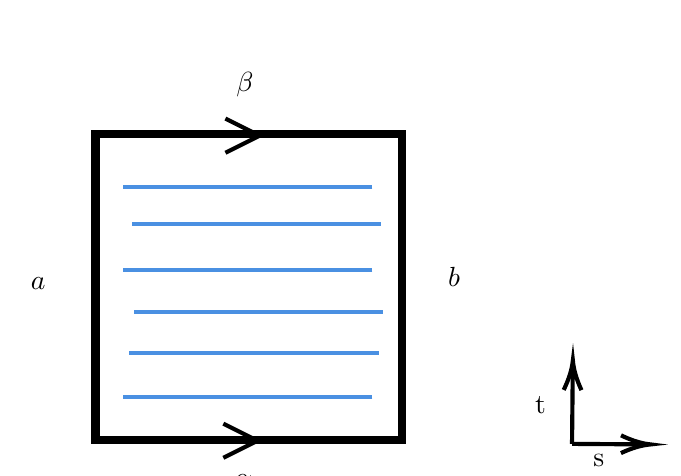
\begin{tikzpicture}[x=0.75pt,y=0.75pt,yscale=-1,xscale=1]
%uncomment if require: \path (0,300); %set diagram left start at 0, and has height of 300

%Shape: Square [id:dp8405561290457572] 
\draw  [line width=3]  (237.48,65) -- (385,65) -- (385,212.52) -- (237.48,212.52) -- cycle ;
%Straight Lines [id:da8154443482370679] 
\draw [line width=1.5]    (467,214.26) -- (467.37,177.1) ;
\draw [shift={(467.4,174.1)}, rotate = 90.57] [color={rgb, 255:red, 0; green, 0; blue, 0 }  ][line width=1.5]    (14.21,-4.28) .. controls (9.04,-1.82) and (4.3,-0.39) .. (0,0) .. controls (4.3,0.39) and (9.04,1.82) .. (14.21,4.28)   ;
%Straight Lines [id:da08150819904971096] 
\draw [line width=1.5]    (467,214.26) -- (501.79,214.5) ;
\draw [shift={(504.79,214.52)}, rotate = 180.4] [color={rgb, 255:red, 0; green, 0; blue, 0 }  ][line width=1.5]    (14.21,-4.28) .. controls (9.04,-1.82) and (4.3,-0.39) .. (0,0) .. controls (4.3,0.39) and (9.04,1.82) .. (14.21,4.28)   ;
\draw  [line width=1.5]  (299,204.52) -- (315.48,212.76) -- (299,221) ;
\draw  [line width=1.5]  (300,57.52) -- (316.48,65.76) -- (300,74) ;
%Straight Lines [id:da7151226501077709] 
\draw [color={rgb, 255:red, 74; green, 144; blue, 226 }  ,draw opacity=1 ][line width=1.5]    (370.79,191.52) -- (250.79,191.52) ;
%Straight Lines [id:da40986873063819407] 
\draw [color={rgb, 255:red, 74; green, 144; blue, 226 }  ,draw opacity=1 ][line width=1.5]    (373.79,170.52) -- (253.79,170.52) ;
%Straight Lines [id:da5100479079903827] 
\draw [color={rgb, 255:red, 74; green, 144; blue, 226 }  ,draw opacity=1 ][line width=1.5]    (375.79,150.52) -- (255.79,150.52) ;
%Straight Lines [id:da23706101064057428] 
\draw [color={rgb, 255:red, 74; green, 144; blue, 226 }  ,draw opacity=1 ][line width=1.5]    (370.79,130.52) -- (250.79,130.52) ;
%Straight Lines [id:da24393778612763894] 
\draw [color={rgb, 255:red, 74; green, 144; blue, 226 }  ,draw opacity=1 ][line width=1.5]    (374.79,108.52) -- (254.79,108.52) ;
%Straight Lines [id:da882868137340323] 
\draw [color={rgb, 255:red, 74; green, 144; blue, 226 }  ,draw opacity=1 ][line width=1.5]    (370.79,90.52) -- (250.79,90.52) ;

% Text Node
\draw (476,218) node [anchor=north west][inner sep=0.75pt]   [align=left] {s};
% Text Node
\draw (448,190) node [anchor=north west][inner sep=0.75pt]   [align=left] {t};
% Text Node
\draw (303,228) node [anchor=north west][inner sep=0.75pt]   [align=left] {$\displaystyle \alpha $};
% Text Node
\draw (304,34) node [anchor=north west][inner sep=0.75pt]   [align=left] {$\displaystyle \beta $};
% Text Node
\draw (205,133) node [anchor=north west][inner sep=0.75pt]   [align=left] {$\displaystyle a$};
% Text Node
\draw (406,128) node [anchor=north west][inner sep=0.75pt]   [align=left] {$\displaystyle b$};


\end{tikzpicture}
     \end{center}
\end{figure}

For \(t=0\) we have that \(H_0(s)=\alpha(s)\) hence this is the bottom edge, similarly the top edge is given by \(H_1(s)=\beta(s)\). Now, when \(H_t(0)=a\) which corresponds to the left edge and similarly for the right edge we can consider \(H_t(1)=b\). This is because we take the origin to be the bottom left most corner of the square.
The blue lines represent the paths (deforming) between \(\alpha\) and \(\beta\).

\begin{mdprop}
    Path-homotopy is an equivalence relation on the set of all paths from \(a\) to \(b\).
\end{mdprop}

\begin{proof}
    We prove the axioms of an equivalence relation.
    \begin{itemize}
        \item Reflexive -- \(\alpha \approxeq \alpha\): let \(H(s,t)=\alpha(s)\) for all \(t\).
        \item Symmetric -- \(\alpha \approxeq_F \beta \then \beta\approxeq_H \alpha\): let \(H(s,t) = F(s,1-t)\).
        \item Transitivity: we have that \(\alpha \approxeq_F \beta\) and \(\beta \approxeq_G \gamma\). We need to find a path homotopy \(H\) such that \(\alpha \approxeq_H \gamma\). To do, we can consider to unit square stacked on top of each other:
        \begin{figure}[H]
             \begin{center}
                 \includegraphics[scale=0.5]{./Resources/Homotopy Transitive.png}
             \end{center}
        \end{figure}
        This is now a rectangle with height \(2\) which violates the requirements to be the domain of a homotopy. To rectify, this problem we can squash down the figure and define a homotopy which travels vertically at twice the `speed' to reach \(\beta\). Thus, the homotopy is as follows:
        \[H(s,t) = \begin{cases}
            F(s,2t) &\text{if } t \in \left[ 0,\half \right] \\
            G(s,2t-1) &\text{if } t \in \left[ \half,1 \right].
        \end{cases}\]
        To show that \(H\) is continuous it suffices to show that if \(C\) is a closed subset of \(X\) then \(H\inv(C)\) is a closed subset of \([0,1]\).
    \end{itemize}
\end{proof}

\begin{mdprop}
    If \(\alpha \sim_F \beta\) and \(\alpha'\sim_G \beta'\) then \(\alpha\beta \sim \alpha'\beta'\).
\end{mdprop}

\begin{mdremark}
    By \(\alpha\beta\) we mean the concatenation of paths.
\end{mdremark}

\begin{mdnote}
    In the next section when defining the fundamental group this proposition implies the closure axiom.
\end{mdnote}

\begin{proof}
    We need a homotopy \(H\) such that \(\alpha\beta \approxeq_H \alpha'\beta'\). To find such a homotopy we employ a previous trick: the square domains. Consider the following figure 
    \begin{figure}[H]
         \begin{center}
             \includegraphics[scale=0.5]{./Resources/Homotopy Closure.png}
         \end{center}
    \end{figure}
    Like before, we need to squash down this domain to a unit square. This is achieved by travelling twice the speed on the \(s\)-axis for \(F\). Therefore, 
    \[H(s,t) =\begin{cases}
        F(2s,t) &\text{if } s\in\left[ 0,\half \right]\\
        G(2s-1,t) &\text{if } s\in \left[ \half,1 \right],
    \end{cases}\]
    noting that \(F(1,t)=x_0=G(1,t)\).
\end{proof}

\subsection{The fundamental group}

\begin{definition}
    The set of all homotopy classes of loops at a given base point \(x_0 \in X\) is denoted by 
    \[\pi_1(X,x_0) = \{[\alpha] : \alpha \text{ is a loop based at }x_0\}.\]
\end{definition}

\begin{mdprop}
    The set \(\pi_1(X,x_0)\) with multiplication \([\alpha][\beta]=[\alpha\beta]\) is a group. We call this the \textbf{fundamental group}.
\end{mdprop}

\begin{proof}
    We prove the group axioms.
    \begin{itemize}
        \item Associativity (i.e. \((\alpha\beta)\gamma \approxeq_H \alpha(\beta\gamma)\)). We need to find such an \(H\). To do so we consider the unit square 
        \begin{figure}[H]
             \begin{center}
                 \includegraphics[scale=0.6]{./Resources/Homotopy associative.png}
             \end{center}
        \end{figure}
        On the bottom, we are travelling \(\alpha\) and \(\beta\) for \(1/4\) of the time then \(\half\) of the time we spend travelling \(\gamma\). Whereas, on the top we travel \(\alpha\) for \(\half\) the time then \(\beta\) and \(\gamma\) for a \(1/4\) of the time. To find a homotopy, we need to find the slope of each line as this will determine the length of the interval and the domain of \(s\) for each path (by rearranging \(t=ms+c\) the equation of the line). Since they must be paths we need to scale and shift the domain of the paths to restrict them to \([0,1]\). To do this, we reparametrise them by \(s \mapsto u(s)\) where 
        \[u(s) = \frac{s -\text{start}(t)}{\text{end}(t)-start(t)}.\] 
        Doing so we have the following homotopy:
        \[H(s,t) = \begin{cases}
            \alpha\left( \frac{4s}{1+t} \right) &\text{if } s\leq \frac{1}{4}(1+t) \\
            \beta(4s-1-t) &\text{if } \frac{1}{4}(1+t)\leq s \leq \frac{1}{4}(2+t) \\
            \gamma\left( \frac{4s-2-t}{2-t} \right) &\text{if } \frac{1}{4}(2+t) \leq s \leq 1.
        \end{cases}\]
        \item Identity: The identity element is the constant path \(\eps(s)=x_0\). If \(\alpha\) is a path \(\eps\alpha\) corresponds to travelling along \(\alpha\) twice the speed and then standing still for the remaining time.
        \item Inverse: The inverse of a path is travelling backwards which is given by \(\alpha(1-s)\).
        We provide the explict stuff below.
        \begin{figure}[H]
             \begin{center}
                 \includegraphics[scale=0.6]{./Resources/Identity and inverse proof of fundamental group.png}
             \end{center}
        \end{figure}
    \end{itemize}
\end{proof}

\subsection{Properties of the fundamental group}

It is natural to doubt the independence of \(\pi_1(X, x_0)\) based on the choice of \(x_0\). But there is
nothing to worry about. Indeed:

\begin{mdprop}
    Suppose that \(X\) is a path connected topological space and let \(x_0,x_1 \in X\) and let \(\sigma\) be a path from \(x_0\) to \(x_1\). The map 
    \[\begin{aligned}
        \phi_{\sigma} :\pi_1(X,x_0) &\to \pi_1(X,x_1) \\
        [\alpha] &\mapsto [\sigma\inv\alpha\sigma]
    \end{aligned}\]
    is a well-defined map and an isomorphism.
\end{mdprop}

\begin{mdremark}
    This allows us to refer to the fundamental group \(\pi_1(X)\).
\end{mdremark}

\begin{proof}
    The homomorpshim proof is trivial. For bijectivity, the inverse map is given by \(\alpha \mapsto \sigma\alpha\sigma\inv\).
\end{proof}

\begin{lemma}
    For the path defined above, we have the following results:
    \begin{itemize}
        \item If \(\alpha \approxeq \alpha'\) then \(\sigma\inv\alpha\sigma \approxeq \sigma\inv \alpha' \sigma\).
        \item \(\sigma\inv (\alpha\beta) \sigma \approxeq (\sigma\inv \alpha\sigma)(\sigma\inv\beta\sigma)\).
    \end{itemize}
\end{lemma}

\begin{proof}
    This is clear since \(\sigma\approxeq \sigma\) etc.
\end{proof}

\subsection{Functoriality}

\begin{mdnote}
    In this section we discuss the following idea, suppose \(X\) and \(Y\) are topological spaces and \(f:X \to Y\) is a continuous function, can we relate the fundamental groups of \(X\) and \(Y\)?
\end{mdnote}

\begin{definition}
    Suppose that \(X\) and \(Y\) are topological space and \(f:X\to Y\) is continuous. The \textbf{induced mapping} on the fundamental group is 
    \[\begin{aligned}
        f_*:\pi_1(X,x_0)&\to \pi_1(Y,y_0), \quad \text{where } y =f(x_0) \\
        [\alpha] &\mapsto [f\circ \alpha].
    \end{aligned}\]
\end{definition}

\begin{lemma}
    Some properties:
    \begin{itemize}
        \item \(f_*\) is a group homomorpshim;
        \item \(\id_*=\id\);
        \item \((g \circ f)_*=g_*\circ f_*\).
    \end{itemize}
\end{lemma}

\begin{mdcor}
    If \(X\) is homeomorphic to \(Y\) then \(\pi_1(X) \cong \pi_1(Y)\).
\end{mdcor}

\begin{mdremark}
    The converse is not true, as the fundamental groups of a point and sphere are both trivial but clearly not homeomorphic.
\end{mdremark}

\begin{corollary}
    If \(X\) is homeomorphic to \(Y\) (often written \(X \approx Y\)) then \(\pi_1(X) \cong \pi_1(Y)\).
\end{corollary}

\subsection{Simply-connected spaces}

\begin{definition}
    A topological space \(X\) is \textbf{simply-connected} if it is path-connected and \(\pi_1(X)=\{e\}\) (i.e. the fundemental group is trivial).
\end{definition}

\begin{example}
    The space \(\RR^n\) homotopic to a point.
\end{example}

\subsection{Fundamental group of a graph}

\begin{figure}[H]
     \begin{center}
         \includegraphics[scale=0.7]{./Resources/Fundamental group of graph.png}
     \end{center}
\end{figure}

\section{Covering spaces}

\begin{definition}
    Let \(Z\) and \(X\) be topological space. The map \(p:Z \to X\) is said to be a \textbf{covering map} if each point \(x \in X\) lies in some open set \(U\) for which the pre-image \(p\inv(U)\) is a  disjoint union of open subsets \(V_i\) of \(Z\) such that the map \(p\mid_{V_i} : V_i \to U\) is a \ul{homeomorphism}. 
\end{definition}

\begin{mdnote}
    The \(V_i\) are \textbf{sheets} of the covering and for each \(x\in X\) the set \(p\inv(x)\) is called the \textbf{fibre} of \(x\).
\end{mdnote}

\begin{proposition}
    We can say \(X\) is a quotient of \(Z\) since this map must be surjective by definition. Moreover, the topology on \(X\) is precisely the quotient topology \(Z/\sim\) where \(x\sim y\) if \(p(x)=p(y)\).
\end{proposition}

\begin{mdexample}
    Some examples:
    \begin{itemize}
        \item \(p:\RR \to S^2\) defined by \(p(s)=e^{2\pi i s }=(\cos 2\pi s,\sin 2\pi s)\);
        \item \(p:S^1 \to S^1\) where \(p(z)=z^k\) and \(\abs{z}=1\) for \(z\in \CC\) and \(k\in \ZZ\);
        \item Let \(\wt{S^n} = \left\{ [v] :v\in S^n \right\}\)  wehre \(v\sim v'\) if \(v=-v'\). This corresponds to the topological space of \(1\)-dimensional linear subspaces of \(\RR^n\). So \(S^n\) is a \textbf{double cover} of \(\wt{S^n}\) in the sense that \(p:S^n \to \wt{S^n}\) is a \(2:1\) map. The quotient \(S^n/\sim\) is the definition of \(\RR\mathbb{P}^n\).
    \end{itemize}
\end{mdexample}

\begin{mdnote}
    From now on `map' means `continuous mapping'.
\end{mdnote}

\begin{definition}
    Given a covering map \(p:Z \to X\) and a continuous map \(f:Y\to X\), a \textbf{lift} of \(f\) is any map \(\wt{f}: Y\to Z\) such that
    \[f = p\circ \wt{f}\]
    That is, it makes the following diagram commute (at any point you start you reach the same endpoint).
    \begin{figure}[H]
         \begin{center}
             \includegraphics[scale=0.75]{./Resources/Lift comm diagram.png}
         \end{center}
    \end{figure}
\end{definition}

\begin{mdprop}
    Given a covering map \(p:Z \to X\) and a map \(f:Y \to X\) if \(Y\) is connected then, any two lifts \(f_1,f_2:Y\to Z\) that agree on one point are equal.
\end{mdprop}

\begin{mdnote}
    That is, if \(f_1(y_0)=f_2(y_0)\) for some \(y_0 \in Y\) then \(f_1 \equiv f_2\).
\end{mdnote}

\begin{proof}
    Suppose \(f_1(y_0) =f_2(y_0)\) for some \(y_0 \in Y\). Consider the subset 
    \[A = \left\{ y\in Y :f_1(y)=f_2(y) \right\},\]
    clearly, \(y_0 \in A\). Let \(y \in A\) then \(f_1(y) \in V_i\) for some \(i\). Sice \(p:V_i \to U\) is a bijection we have that \(f_1\) and \(f_2\) must agree on the entire open set so 
    \[f_1\inv(V_i)=f_2\inv(V_1)=f\inv(U).\]
    It follows that \(A\) is an open subset of \(Y\) and that \(Y\setminus A\) is also open since \(Y=A\) is connected.
\end{proof}

\begin{mdthm}
    Fix \(x_0 \in X\) and \(z \in p\inv(x_0)\). Let \(\alpha,\beta :[0,1] \to X\) be equivalent loops based at \(x_0\) (i.e. \(\alpha \approxeq \beta\)). Then
    \begin{enumerate}
        \item \(\alpha\) has a unique lift \(\wt{\alpha}_z :[0,1]\to Z\) such that \(\wt{\alpha}(0)=z\).
        \item Let \(F : [0,1] \times [0,1] \to X\) be the path homotopy for \(\alpha\approxeq_F \beta\) then, \(F\) has a unique lift \(\wt{F}:[0,1]\times[0,1] \to Z\) such that \(\wt{F}_0 = \wt{\alpha}_z\).
    \end{enumerate}
    Equivalently, the following diagrams commute 
    \[\begin{tikzcd}
        & Z &&& Z \\
        {[0,1]} & X && {[0,1]\times[0,1]} & X
        \arrow["\alpha"', from=2-1, to=2-2]
        \arrow["{\exists!\widetilde{\alpha}_z}", dashed, from=2-1, to=1-2]
        \arrow["p", from=1-2, to=2-2]
        \arrow["F"', from=2-4, to=2-5]
        \arrow["{\exists!\widetilde{F}}", dashed, from=2-4, to=1-5]
        \arrow["p", from=1-5, to=2-5]
    \end{tikzcd}\]
\end{mdthm}

\begin{mdnote}
    We have applied the proposition above to \(Y=[0,1]\) and \(f=\alpha\) (a loop or path).
\end{mdnote}


\begin{corollary}
    The endpoint \(\wt{\alpha}_z(1)\) of \(Z\) depends only on the class \([\alpha]\) of \(\alpha\) in \(\pi_1(X,x_0)\), so fixing \(z\) determines a map \(\pi_1(X,x_0)\to p\inv(x_0)\).
\end{corollary}

\section{Groups acting on sets}

\begin{definition}
    Let \(G\) be a group and \(\Omega\) any set. A \textbf{right action} of \(G\) on \(\Omega\) is a mapping 
    \[\begin{aligned}
        \Omega \times G &\to \Omega \\
        (z,g) &\mapsto z\cdot g
    \end{aligned}\]
    such that 
    \begin{itemize}
        \item \(z\cdot e =z\),
        \item \(z\cdot (gh)= (z\cdot g) \cdot h\) for all \(z\in \Omega\) and \(g,h \in G\).
    \end{itemize}
\end{definition}

\begin{mdremark}
    If \(\abs{\Omega}=n\) this means that there is a group homeomorphism \(G \to S_n\).
\end{mdremark}

\begin{definition}
    Fix \(z \in \Omega\) then \(G_z = \left\{ g\in G :z\cdot g =z \right\}\) is a subgroup of \(G\), called the \textbf{stabiliser} of \(z\). 
\end{definition}

\begin{lemma}
    If \(g \mapsto z\cdot g\) it identfies the set \(\left\{ G_zg :g \in G \right\}\) of right cosets in \(\Omega\).
\end{lemma}

\begin{mdthm}[Action of \(\pi_1\) on a fibre]
    Let \(p:Z \to X\) be a covering map. Fix \(x_0 \in X\) and set 
    \[\begin{aligned}
        G &= \pi_1(X,x_0) \\
        \Omega &= p\inv(x_0).
    \end{aligned}\]
    \begin{enumerate}
        \item Setting \(z\cdot [\alpha]=\wt{\alpha}_z(1)\) defines a right action of \(G\) on \(\Omega\).
        \item If \(z \in p\inv(x_0)\), the induced homomorphism \(p_*:\pi_1(Z,z) \to \pi_1(X,x_0)\) is injective.
        \item The stabiliser \(\left\{ [\alpha] : z\cdot [\alpha]=z \right\}\) is precisely the subgroup \(p_*(\pi_1(Z,z))\) of \(G\).
        \item the map defined in \((1)\) is surjective if \(Z\) is path-connected.
        \item the map defined in \((1)\) bijective if \(Z\) is simply connected.
    \end{enumerate}
\end{mdthm}

\begin{proof}
    We prove each statement in turn.
    \begin{enumerate}
        \item Trivial.
        \item Suppose \(\gamma\) is a loop in \(\wt{X}\) that projects to \(p \circ \gamma\) which is homotopic \(F\) to \(e_{x_0}\), the constant loop. We know this homotopy lifts uniquely to a homotopy \(\wt{F}\) of paths in \(\wt{X}\). As we have seen in the proof of the previous proposition, if two paths \(\alpha \sim \beta\) in \(X\) are homotopic via \(F\) then their respective unique lifts \(\wt{\alpha}, \wt{\beta}\) are homotopic in \(\wt{X}\) via \(\wt{F}\). This means that \(\gamma\) is homotopic via \(\wt{F}\) to the constant loop \(\wt{x}_0\). Hence \(p_*\) has a trivial kernel.
        \item Fix a \(z \in p^{-1}(x_0)\) and suppose \([\alpha]\) is a loop in \(X\) based at \(x_0\) such that its lift \(\wt{\alpha}_z(s)\) starts and ends at \(z\). Clearly this loop projects down to \(\alpha\) so \([\alpha] \in \text{Im}(p_*)\). Conversely, suppose \([\alpha] \in \text{Im}(p_*)\), i.e.: there exists some \(\wt{\alpha}_z(s)\) a loop in \(\wt{X}\) that projects down to \(\alpha\). Thus the action of \([\alpha]\) on \(z\), i.e., \(z \cdot [\alpha]\) is equal to the endpoint of \(\wt{\alpha}_z(s)\), which was \(z\) so \([\alpha]\) belongs to the stabiliser.
        \item Suppose \(z' \in p^{-1}(x_0)\) is given. Choose a path \(\sigma\) from \(z\) to \(z'\) in \(\wt{X}\). The loop \(\alpha = p \circ \sigma\) is based at \(x_0\). By uniqueness of path lifting, \(\wt{\alpha}_z = \sigma\) so \(\wt{\alpha}_z(1) = z'\).
        \item To show bijectivity in case of \(\wt{X}\) being simply connected, we note that if \(z \cdot [\alpha] = z \cdot [\beta]\), by definition of action, we see that \(z \cdot [\alpha\beta^{-1}] = z\) so \([\alpha\beta^{-1}] \in \text{Stab}(z)\). Note that \(\text{Stab}(z)\) is isomorphic to \(\pi_1(\wt{X}) = \{1\}\), which implies \([\alpha] = [\beta]\).
        \(\square\)
    \end{enumerate}
\end{proof}

\subsection{Fundamental group of a circle}

\begin{mdcor}
    \(\pi_(S^1,1) \cong \ZZ \cong \mathbb{F}_1\).
\end{mdcor}

\begin{proof}
    We apply the theorem above with the covering map 
    \[\begin{aligned}
        p:\RR &\to S^1 \subset \CC \\
        s &\mapsto (\cos(2\pi s),\sin(2\pi s))
    \end{aligned}\]
    we fix the point \((1,0) \in S^1\) and notice that the fibre \(p\inv((1,0))=\ZZ\). The path \(s\mapsto sn\) in \(\RR\) projects to the loop \(\alpha_n :s \mapsto \exp(2\pi isn )\) in \(S^1\) adn \(0\cdot [\alpha_n]=n\).
\end{proof}

\subsection{Example of covering spaces}

\subsubsection{Torus to Klein bottle}

\begin{mdprop}
Consider the torus and the Klein bottle as quotients of the unit square with their respective boundary codes. Let the quotient maps be 
\[q_T :[0,1] \times [0,1] \to \mathbb{T} \quad \text{and} \quad q_K :[0,1] \times [0,1] \to \mathbb{K}\]
respectively.

The map \(p:\mathbb{T} \to \mathbb{K}\) defined by 
    \[p(q_T(s,t))= \begin{cases}
        q_K(2s,t) &\text{if } s\leq \half \\
        q_K(2s-1,1-t) &\text{if } s\geq \half
    \end{cases}\]
    is a \ul{double covering space}.
\end{mdprop}

\begin{mdprop}
    \(\pi_1(\mathbb{T},x_0) \cong \pi_1(S_1\times S_1)\cong \ZZ^2\).
\end{mdprop}

\subsubsection{Sphere and real projective plane}

As we saw before, \(S^n\) is a double cover of \(\mathbb{RP}^n\). Given a point \(x_0 \in \mathbb{RP}^n\), its fiber consists of two elements, namely \(x_0\) and \(-x_0\). This also holds for what we have understood so far as \( \mathbb{RP}^2\). Noting that \(S^2\) is simply connected (This is also true if \(n > 2\)), it follows that there is a bijection between elements of \(\pi(\mathbb{RP}^2, x_0)\) and \(\{x_0, -x_0\}\). There is only one group of order 2, hence
\[
\pi_1(\mathbb{RP}^2) \cong \mathbb{Z}/2\mathbb{Z}
\]

\section{Free Groups}

We know what a free group is.

\begin{theorem}
    The free group on one generator (letter) is the infinite cyclic group 
    \[\mathbb{F}_1 = \langle x \rangle = \{x^n : n \in \ZZ\} \cong (\ZZ,+).\]
\end{theorem}

\begin{definition}
    Let \(G\) and \(H\) be groups. The \textbf{free product} \(G * H\) is a group whose elements are of the form 
    \[g_1h_1g_2h_2 \cdots \quad \text{where } g_i \in G \text{ and } h_i \in H.\]
\end{definition}

\begin{example}
    The free group with two generators is 
    \[\mathbb{F}_2 = \mathbb{F}_1 * \mathbb{F}_1 = \langle a,b\rangle.\]
    In contrast, the Cartesian product \(\mathbb{F}_1 \times \mathbb{F}_1\) is not \textbf{free}.
\end{example}

\subsection{Group presentation}

\begin{definition}
    A \textbf{commutator} of \(a,b\) denoted by \([a,b]=aba\inv b\inv\). 
\end{definition}

\begin{definition}
    Presentation of group -- trivial from project. From \(\langle X \mid R \rangle\) we call elements of \(R\) \textbf{relators}.
\end{definition}

\begin{theorem}
    We have that \([b,a]=[a,b]\inv\) and \([a,b\inv]=b\inv[b,a]b\).
\end{theorem}

\begin{theorem}
    Any group \(G \cong F/N\) where \(F\) is a free group and \(N\) is the smallest normal subgroup containing all the relators.
\end{theorem}

\begin{mdprop}[Nielsen-Schreier]
    We have the following:
    \begin{enumerate}
        \item Any subgroup of a free group is free, but in general any of the relators will not generate \(N\).
        \item If \(F_n/N\) is finite of size \(i\) then \(N \cong F_{i(n-1)+1}\).
    \end{enumerate}
\end{mdprop}

\begin{mdexample}
    Let \(K\) be a (left or right) trefoil knot in \(\RR^3\). The Wirtinger presentation of \(G = \pi_1(\RR^3 \setminus K)\) is given by 
    \[G = \langle \alpha,\beta,\gamma \mid \alpha\inv \beta\alpha\gamma\inv, \beta\inv\gamma\beta\alpha\inv, \gamma\inv\alpha\gamma\beta\inv\rangle,\]
    with one relation for each crossing. 
    We can simplify the relation by eliminating \(\gamma\) and settign \(a=\alpha\beta\) and \(b=\alpha\beta\alpha\) to obtain 
    \[G = \langle a,b \mid a^3b^{-2} \rangle.\]
\end{mdexample}

\section{The Van Kampen Theorem}

\begin{mdnote}
    Before stating the theorem we intrdouce a definition of the wegde sum.
\end{mdnote}

\begin{definition}
    Let \(X\) and \(Y\) be topological spaces with \(x_0 \in X\) and \(y_0 \in Y\). The \textbf{wedge sum} of \(X\) and \(Y\) is 
    \[X\vee Y = (X \sqcup Y)/\sim\]
    where \(\sim\) is the equivalence relation which identifies \(x_0\) with \(y_0\) and vice versa.
\end{definition}

\begin{mdnote}
    In simpler terms, think of the wedge sum as a way of combining two spaces by sticking them together at a single point. Imagine you have two separate shapes, like a circle and a triangle. The wedge sum lets you join them together at one point, like gluing the tip of the triangle to the edge of the circle.
\end{mdnote}

\begin{mdexample}
    \begin{figure}[H]
         \begin{center}
             \includegraphics[width=\textwidth]{./Resources/Wedge example.png}
         \end{center}
    \end{figure}
\end{mdexample}

\subsection{Homotopy of maps and spaces}

\begin{definition}[Homotopy of maps]
    Two \textbf{maps} \(f_0,f_1 : X\to Y\) are \textbf{homotopic}, denoted by \(f_0 \simeq f_1\) if there exists a map 
    \[H:X \times [0,1] \to Y \text{ such that \(H(x,0)=f_0\) and \(H(x,1)=f_1\).}\]
\end{definition}

\begin{definition}[Homotopy of spaces]
    Let \(X,Y\) be path-connected. The \textbf{spaces} \(X,Y\) are called \textbf{homotopic}, denoted by \(X \simeq Y\) if there exists maps \(f:X \to Y\) and \(g : Y\to X\) such that 
    \[g \circ f \simeq \id_X \quad \text{and} \quad f\circ g \simeq \id_Y.\]
\end{definition}

\begin{definition}
    Let \(X,Y\) be path-connected. If \(X \subset Y\) then \(X\) is called a (strong) \textbf{deformation retract} of \(Y\) if \(f\) is the inclusion map, 
    \[g\circ f \simeq \id_X \quad \text{and} \quad f \circ g \simeq \id_Y\]
    with homotopy \(H(t,x)=x\) for all \(x \in X\).
\end{definition}

\begin{mdexample}
    \(S^1\) is a deformation retract of \(\CC\setminus \left\{ 0 \right\}\). We can take \(g(z)=\frac{z}{\abs{z}}\) and \(H(z,t)=\frac{(1-t) z}{\abs{z}}+tz\).
\end{mdexample}

\begin{mdprop}
    If \(X \simeq Y\) then \(\pi_1(X) \cong \pi_1(Y)\).
\end{mdprop}

\subsection{The theorem}

The Van Kampen theorem will allow us to compute the fundamental group of a space which is the union of two open subsets \(U,V\) with path-connected intersection. We can express these conditions with the following commutative diagram:

\begin{figure}[H]
     \begin{center}
         \includegraphics[scale=0.75]{./Resources/VK sets.png}
     \end{center}
\end{figure}

\noindent These maps are continuous and so by the functoriality of the fundamental group they all induce group homomorpshims:

\begin{figure}[H]
     \begin{center}
         \includegraphics[scale=0.75]{./Resources/VK induced.png}
     \end{center}
\end{figure}

\begin{mdthm}[Seifert-Van Kampen]
    Let \(X = U \cup V\) be a topological space where \(U,V\) and \(U\cap V\) are non-empty, open sets. Let \(K = \pi_1(U \cap V)\).
    \begin{enumerate}
        \item If \(U \cap V\) is simply-connected then \(\pi_1(X) \cong \pi_1(U) * \pi_1(V)\).
        \item If \(U \cap V\) path-connected then 
        \[\pi_1(X) \cong \pi_1(U) *_K \pi_1(V) = (\pi_1(U) * \pi_1(V))/N\]
        where \(N\) is the smallest normal subrgoup containing all elements \(i^*(k)\inv j_*(k)\) for \(k \in K\).
    \end{enumerate}
\end{mdthm}

\begin{mdexample}[VK2]
    Take \(X = T\). Let \(o\) be the centre of the square \(\mathcal{P}\), \(\hat{o}\) its image in \(T = \hat{\mathcal{P}}\), and \(U = T\setminus\{\hat{o}\}\). Then \(U\) retracts to the boundary \(\partial\mathcal{P}\) of the unique face of \(T\), and 

\[ U \simeq \partial\mathcal{P} \Rightarrow \pi_1(U) \simeq \pi_1(\partial\mathcal{P}) \simeq F_2. \]

Now take \(V\) to a small open disk (or square) containing \(\hat{o}\). Then \(U \cap V\) is homotopic to \(\partial\mathcal{P}\) and a circle, and \(i_*\) maps the generator of \(\pi_1(U \cap V)\) to the class \(aba^{-1}b^{-1}\) in \(\pi_1(U)\), whilst \(\pi_1(V) = \{e\}\) is trivial. Therefore \(N\) is the smallest normal subgroup of \(\pi_1(U) * \pi_1(V)\) containing \(aba^{-1}b^{-1}\), and \(\pi_1(T) \simeq \langle a, b \mid aba^{-1}b^{-1}\rangle\).
\end{mdexample}


\begin{mdexample}[VK2]
    In the description of a torus \( T \) as the quotient of a square \( \mathcal{P} \), its boundary \( \partial\mathcal{P} \) maps to the `wedge' \( S^1 \vee S^1 \) of two circles, homeomorphic to the figure-eight. Call this space \( X \). 
    
    The circles can be enlarged into open sets \( U, V \) with \( U \simeq S^1 \), and \( U \cap V \) a `cross'. This cross is homotopic to a point: the arcs can be continuously shortened until the figure has been collapsed to the central vertex \( v \). This point is a deformation retract of the cross; one says that \( U \cap V \) \textbf{retracts} to \( v \).
    
    Then VK1 and the previous proposition imply that
    \[ \pi_1(S^1 \vee S^1) \simeq \pi_1(S^1) * \pi_1(S^1) \simeq F_1 * F_1 = F_2. \]
    If we regard the figure-eight \( X \) as a graph, then \( \{v\} \) is itself a minimal spanning tree (MST). It's a general result that the fundamental group of a graph is isomorphic to \( F_n \), where \( n = E - (V - 1) \) is the number of edges not in a MST.
\end{mdexample}

\subsection{The fundamental group of spheres}

\begin{mdthm}
    We have that \(S^n\) is simply connected if \(n\geq 2\) i.e.\ \(\pi_1(S^n)\cong \{e\}\).
\end{mdthm}

\begin{proof}
    One proof exploits the fact that \(S^n\) minus a point is homeomorphic to \(\mathbb{R}^n\). Any loop in \(S^n\) can then be regarded as a loop in \(\mathbb{R}^n\) based at the origin, and \(H(s, t) = (1 - t)\alpha(s)\) deforms it to the constant loop.
    
    Fix \(n \geq 2\). Then \(S^n\) is the union of \(3/4\)-spheres
\[
U = \left\{ (x_1, \ldots, x_{n+1}) : \sum x_i^2 = 1, x_{n+1} \geq -\frac{1}{2} \right\}
\]
\[
V = \left\{ (x_1, \ldots, x_{n+1}) : \sum x_i^2 = 1, x_{n+1} \leq \frac{1}{2} \right\},
\]
each homeomorphic to a disk, and simply connected. The `equator' \(x_{n+1} = 0\) can be identified with \(S^{n-1}\), and is path-connected for \(n \geq 2\). By Theorem vK2, \(\pi_1(S^n)\) is a quotient of the free group \(F = \pi_1(U) * \pi_1(V) = \{e\}\), and therefore trivial. 

\end{proof}

\begin{mdremark}
    If we accept that \(S^2\) is simply connected, we can deduce by induction that \(S^n\) is for \(n \geq 3\), using only vK1. For the equator \(S^{n-1}\) above is a deformation retract of \(U \cap V\). So now all of \(U\), \(V\), \(U \cap V\) are simply-connected for \(n \geq 3\).
\end{mdremark}

\subsection{The fundamental group of a surface of genus 3}

\begin{figure}[H]
     \begin{center}
         \includegraphics[scale=0.9]{./Resources/Fundamental group genus 3.png}
     \end{center}
\end{figure}

\subsection{Summary for fundamental groups of surfaces}

\begin{mdprop}
    If the surface \(\mathcal{M}\)
    \begin{itemize}
        \item is an orientable surface of genus \(g\) with no boundary then 
        \[\pi_1(\mathcal{M}) \cong \langle a_1,\ldots, a_g,b_1,\ldots,b_g \mid \mathbb{A}_g\rangle.\]
        It is abelian \(\iff g=0,1\) i.e. it is the surface is the sphere or torus.
        \item is a non-orientable surface with \(\chi=2-h\) with no boundary then 
        \[\pi_1(\mathcal{M}) \cong \langle c_1,\ldots,c_h \mid c_1^2 \cdots c_h^2 \rangle.\]
        It is abelian (and finite) \(\iff\) \(h=1\) i.e. the surface is the projective plane.
        \item is an orientable surface of genus \(g\) with \(r=1\) boundary component
        \[\begin{aligned}
            \pi_1(\mathcal{M}) &\cong \langle a_1,\ldots,a_g, b_1,\ldots,b_g,d \mid \mathbb{A}_g d\rangle \\
            &\cong \langle a_1,\ldots,a_g, b_1,\ldots,b_g \rangle \\
            &\cong \mathbb{F}_{2g}.
        \end{aligned}\]
    \end{itemize}
\end{mdprop}

\begin{mdnote}
    For the last one, that is because \(d = (\mathbb{A}_g)\inv\).
\end{mdnote}

\section{Knot groups}

\begin{mdnote}
    Let \(K\) be a knot in space, the aim of this section is to describe \(\pi_1(\RR^3\setminus K)\).
\end{mdnote}

\begin{definition}
    We call the set \(\RR^3\setminus K\) the \textbf{knot complement} which is a \(3\)-manifold.
\end{definition}

\begin{proposition}
    \(\pi_1(\RR^3\setminus S^1,x_0) \cong F_1\)
\end{proposition}

\begin{proof}
    Let \(U\) be an unknot represented by \(S^1 \subset \RR^2\subset \RR^3\) and fix a basepoint \(x_0\). An obvious element of \(\pi_1(\RR^3\setminus S_1,x_0)\) is \([\alpha_1]\) where \(\alpha_1\) is a loop wrapping around \(S^1\) once. Therefore, the statement is intuitively clear. Or we can use the Van Kampen theorem to show that 
    \[\begin{aligned}
        \pi_1(\RR^3\setminus S^1) &\cong \pi_1(S^3\setminus S^1) \\
        &\cong \pi_1(S^1).
    \end{aligned}\]
\end{proof}

\begin{mdthm}
    If \(K\) is knot and \(\pi_1(\RR^3\setminus K) \cong F_1\) then \(K\) is ambient isotopic to an unknot.
\end{mdthm}

\begin{mdprop}
    The \textbf{knot group} is generated by the loops \(\alpha_1,\ldots,\alpha_c\) subject to any \(c-1\) of the crossing relations
    \[[\alpha_i][\alpha_j][\alpha_i]\inv =[\alpha_k]\] 
    where \(c\) is the number of crossings (hence, arcs) of a knot diagram.
\end{mdprop}

\begin{proposition}
    For a torus knot type \((p,q)\) (\(\gcd(p,q)=1\)) we have \(\pi_1(\RR^3\setminus K)\cong \langle a,b \mid a^p b^{-q} \rangle\).
\end{proposition}

\begin{mdexample}
    The trefoil is a torus knot \((p,q)=(3,2)\).
\end{mdexample}

\begin{example}
    What a torus knot looks like:
    \begin{figure}[H]
         \begin{center}
             \includegraphics[scale=0.5]{./Resources/Torus knot.png}
         \end{center}
    \end{figure}
\end{example}

\pagebreak

\appendix

\addcontentsline{toc}{section}{Appendix}
\section*{Appendix}

\section{YouTube Material}

\href{https://youtube.com/@richardhepworth1441?si=FlN-NyqyRQ6juq87}{Richard Hepworth}

\section{Left and Right Trefoil Knot}

Below is an image of the LEFT trefoil knot 

\begin{center}
    \includegraphics[scale=0.5]{./Resources/left trefoil.svg.png}
\end{center}

Below in an image of the RIGHT trefoil know 

\begin{center}
    \includegraphics[scale=0.5]{./Resources/Right trefoil.svg.png}
\end{center}


\end{document}